%% Page settings.
\documentclass[12pt,a4paper,twoside]{article}
\usepackage[top=1in, left=1in, bottom=1in, right=1in]{geometry}
\renewcommand{\baselinestretch}{1.5}
%==================================================%
%% Encoding packages.
\usepackage[UKenglish]{babel}
\usepackage[nodayofweek]{datetime}
\usepackage[T1]{fontenc}
\usepackage[utf8]{inputenc}
\usepackage{amsmath}
\usepackage{amsthm}
\DeclareMathAlphabet\mathbb{U}{msb}{m}{n}
%\usepackage{amsfonts}
\usepackage{amssymb}
\usepackage{calc}
\usepackage{natbib}
\usepackage{color}
\usepackage{subcaption}
\usepackage{caption}
%\usepackage{subfig}
\setlength{\headheight}{15pt}
%==================================================%
%% Document details.
\usepackage{titling}
\title{Information and admissible sets}
\author{Jeff Rowley}
\newcommand{\thedate}{\today}
% Enter document details here.
\newcommand{\details}{C:/Dropbox/TeXTemplates/}
% Enter the file path here for the UCL logo and bibliography.
% Change this file path for different computer systems.
\newcommand{\homePC}{C:/Users/Jeffro/Documents/}
\newcommand{\workPC}{U:/}
%==================================================%
%% Date macro.
\newcommand{\theseason}[1]{
\ifcase \month 
\or Winter\or Winter\or Spring\or Spring\or Spring\or Summer\or Summer\or Summer\or Autumn\or Autumn\or Autumn\or Winter\fi}
% Displays the season.
% Obsolete in this template.
%==================================================%
%% Useful packages.
\usepackage{enumerate}		% Lists.
\usepackage{bbm}			% Indicator functions.
\usepackage{lipsum}			% Random text generator.
\usepackage{MnSymbol}		% Arrows.
\usepackage{graphicx}		% Graphics.
\usepackage{mathtools}		% Math*lap command.
 \usepackage{booktabs}
 \usepackage{multirow}
 \usepackage{rotating}
 \usepackage{anyfontsize}
%==================================================%
%% Theorem environments.
\newcounter{countthm}[section]
\newcounter{countlem}[section]
\newcounter{countex}[section]
% Creates new counters which reset at each new section. 
\renewcommand{\thecountthm}{\thesection.\arabic{countthm}}
\renewcommand{\thecountlem}{\thesection.\arabic{countlem}}
\renewcommand{\thecountex}{\thesection.\arabic{countex}}
% Redefines counters to include the section number.
\newtheorem{thm}[countthm]{Theorem}
% Creates a theorem environment - type \thm to begin.
\newtheorem{lem}[countlem]{Lemma}
% Creates a lemma environment - type \lem to begin.
\newtheorem{ex}[countex]{Example}
% Creates an example environment - type \ex to begin.
\newtheorem*{Acknowledgements}{Acknowledgements}
% Creates a thanks environment.
\newcommand{\newthm}[1]{\newtheorem*{#1}{#1}}
% A macro that makes defining new theorem environments quick.
% Type \newthm{<Theorem name here>} to begin.
%==================================================%
%% Math operators.
\DeclareMathOperator*{\plim}{plim}
% Writes plim in math environment - type \plim to enter.
\DeclareMathOperator*{\argmax}{argmax}
% Writes argmax in math environment - type \argmax to enter.
\DeclareMathOperator*{\argmin}{argmin}
% Writes argmin in math environment - type \argmin to enter.
\DeclareMathOperator*{\argsup}{argsup}
% Writes argsup in math environment - type \argsup to enter.
\DeclareMathOperator*{\arginf}{arginf}
% Writes arginf in math environment - type \arginf to enter.
\newcommand\independent{\protect\mathpalette{\protect\independenT}{\perp}} 
\def\independenT#1#2{\mathrel{\rlap{$#1#2$}\mkern2mu{#1#2}}} 
% Pastes an independence symbol - type \independent to enter.
\DeclareMathOperator*{\generates}{:.}
% Write generate symbol (identification).
\DeclareMathOperator*{\generated}{.:}
% Write generated symbol (identification).
\DeclareRobustCommand{\stirling}{\genfrac\{\}{0pt}{}}
% Stirling number of the second kind.
\DeclareMathOperator*{\card}{card}
%==================================================%
%% Abbreviations.
\newcommand{\US}{United States}
% Use \US macro when use is as a noun.
% Use U.S. when use is as an adjective.
%==================================================%
%% Equation numbering.
\numberwithin{equation}{section}
% Numbers equations up to the subsection. To change level,
% replace subsection with section.
%==================================================%
%% Counters.
\newcounter{saveenumi}
\newcounter{saveenumi1}
\setcounter{section}{0}
\newcommand\invisiblesection[1]{%
  \refstepcounter{section}%
  \addcontentsline{toc}{section}{\protect\numberline{\thesection}#1}%
  \sectionmark{#1}}
%==================================================%
\newcommand{\ESRC}{I gratefully acknowledge financial support from the Economic and Social Research Council (ESRC).}
\newcommand{\RLaTeX}{I acknowledge the \emph{R} and \emph{\LaTeX} communities, and the wealth of knowledge that they have made freely available to all.}
\newcommand{\Art}{Artstein's Inequality}
%==================================================%
%% The title page.
\makeatletter				
% Changes @ to catcode 11.
\renewcommand{\@maketitle}{
\null
\graphicspath{ {\details} }
\flushleft{\includegraphics[width=40mm]{UCL_Logo_Orange}}
\hspace{5mm}
\normalsize Department of Economics, University College London\\
\vskip\bigskipamount
\leaders\vrule width \textwidth\vskip0.4pt 
\vskip\bigskipamount 
\nointerlineskip
% This completes the UCL banner.
\begin{center}
\begin{minipage}{100mm}
\begin{center}
\vspace{20mm}
\LARGE
\textbf{
\@title}
\par
\vspace{10mm}
\normalsize
\@author
\par
\vspace{5mm}
\normalsize
\thedate
\end{center}
\end{minipage}
\end{center}
}
\makeatother				
% Reverts @ to catcode 12.
%==================================================%
%% Packages to load at end of preamble. 
% Note conflict between Tkz-euclide package set and 
% game theory package set. Load one or the other.
\usepackage{hyperref}
%\usepackage[numbered]{mcode}

%% Tkz-euclide package set.
%\usepackage{tkz-euclide}
%\usepackage{pgfplots}
%\usepgfplotslibrary{external} 
%\tikzexternalize[prefix=tikz/]

%% Game theory package set.
\usepackage{pstricks}	
\usepackage{egameps}		 
\usepackage{pst-3d}			
\usepackage{sgame}	
\renewcommand{\gamestretch}{1.5}
%==================================================%
%% Further notes regarding egameps package.
% The egameps package is incompatible with this template
% due to UCL logo. Solution is to independently run 
% egameps through on a latex blank document, then insert 
% pdf into this document. Recall that to run egameps:
% "latex" --> "DVi->PS" --> "PS->PDF"
% then use "includegraphics[]" with trim option. 
%==================================================%
%% Headers and footers.
\usepackage{fancyhdr}
\pagestyle{fancy}
\renewcommand{\sectionmark}[1]{\markright{\thesection.\ #1}}
% This redefines the \rightmark command so that the section number does not appear.
% NOTE: To remove the section number, delete <<\thesection.\>>
\lhead[\thepage]{\rightmark}
\rhead[\rightmark]{\thepage}
\chead[]{}
\cfoot[]{}
%\lfoot[\thetitle]{}
%\rfoot[]{\theauthor}
\renewcommand*\thesection{\arabic{section}}
\usepackage{epigraph}
%==================================================%
%% Start of document.
\begin{document}
\maketitle
\vspace{10mm}
\begin{abstract}
\noindent <<Abstract here>>
\begin{Acknowledgements}
{\RLaTeX} I thank Andrew Chesher and Toru Kitagawa for their supervision and support. I further thank Adam Rosen for helpful discussion. {\ESRC}
\end{Acknowledgements}
\end{abstract}
\vspace{5mm}
%==================================================%
%% Document.
%==================================================%

I study a non-parametric binary choice model with a binary endogenous variable. I explore the effect of incorporating information into the model on the identified set of the average causal effect of the endogenous variable on the outcome variable. The model embeds an exclusion restriction and an independence restriction that together define an instrumental variable but is silent as to the relationship between the endogenous variable and the instrumental variable. I restrict the relationship between the outcome variable and the endogenous variable up to a non-parametric threshold crossing function. The model is credible \citep{book.manski} in that it embeds restrictions that impose weaker constraints on assumed behaviour, but does not identify the average causal effect of the endogenous variable on the outcome variable.\footnote{Assumptions that cannot be tested using data. The model does embed some non-trivial non-verifiable restrictions that might be relaxed.} Rather, the model partially identifies the average causal effect of the endogenous variable on the outcome variable. 

I define information to be those additional characteristics of economic agents that are observable with the caveat that these characteristics are exogenous and are relevant to the latent structure. It is convenient to think of such characteristics as being predetermined and immutable; characteristics that result from choices that are made jointly with the outcome variable are excluded by the definition. Accordingly, exogenous variables and instrumental variables are each regarded as information, and I distinguish between these classes of information. I study how the the identified set of the average causal effect of the endogenous variable on the outcome variable changes as each class of information is incorporated into the model separately. 

It is useful to distinguish between classes of information since each class enters the latent structure in a different way. Exogenous variables are permitted to enter the structural equation for the outcome variable and to determine the endogenous variable. As such, exogenous variables can be seen to enrich both individual response and individual selection, respectively. An important consequence is that the causal effect of the endogenous variable on the outcome variable depends upon the values of exogenous variables when individual response is enriched. In contrast, instrumental variables are excluded from the structural equation for the outcome variable by definition and so only enrich individual selection. Given this, the effect of incorporating information is different depending upon the class of information that is being incorporated into the model.  

Incorporating information of either class is generally sensible for a number of reasons. Firstly, incorporating information is known to be efficient; variation that is attributable to an observable variable is instead attributable to unobservable heterogeneity when that variable is omitted. Secondly, the effect of incorporating information for partially identifying models is not well-documented. In identifying models, if an omitted variable is a determinant of the endogenous variable then its effect on the outcome variable is instead attributable to the endogenous variable, and is a bias. A contribution that I make is in showing that incorporating information negates this bias, and is equivalent to a shift in the location of the estimate of the identified set. A further reason to particularly favour incorporating exogenous variables is that the average causal effect of the endogenous variable on the outcome variable in identifiable sub-populations can be recovered. I name this structural characteristic the conditional average causal effect of the endogenous variable on the outcome variable, and index it by the conditioning value.\footnote{The conditioning value is specifically the value of the exogenous variables. \cite{hEvY05} defines a parameter $ATE(x)$ that is equivalent to the conditional average causal effect of the endogenous variable on the outcome variable at the conditioning value $x$. \cite{kHt10} and \cite{13.misc.abrevaya} instead refer to this parameter as the conditional average treatment effect and abbreviate this to $CATE(x)$.} Understanding the effect of an intervention in sub-populations can be interesting if the intervention can be targeted or if the intervention is to be applied elsewhere in a population that differs according to its observable characteristics. 

A relevant question is how to relate conditional causal effects to (unconditional) causal effects. More precisely, how does the average causal effect of the endogenous variable on the outcome variable relate to its conditional counterparts? I show that the average causal effect of the endogenous variable on the outcome variable can be expressed as a Minkowski summation of its conditional counterparts when the non-parametric binary choice model is augmented. I derive sharp bounds on the conditional average causal effect by applying random set theory. 
%I employ the capacity (or containment) functional as in \cite{crs13} as a matter of choice, rather than the Aumann expectation as in \cite{bEmOImOF12}. As I show that the average causal effect of the endogenous variable on the outcome variable can be expressed as a Minkowski summation of its conditional counterparts, I derive sharp bounds on the average causal effect of the endogenous variable on the outcome variable.\footnote{\cite{book.molchanov} is a useful companion in the study of random sets.}     

I demonstrate application of the non-parametric binary choice model, elucidating the practical difficulties that arise when estimating set identifying models (focusing on those issues that arise from incorporating information). As in \cite{cr13}, I estimate the average causal effect of additional children on a mother's employment using US census data. I extend \cite{cr13} in a number of ways. First, I report statistical uncertainty in the estimate of the average causal effect of additional children on a mother's employment using a method that is outlined in \cite{cHlr13}. Second, I enrich the support of the instrumental variable and explore the effect that this has on the estimate of the identified set of values for the average causal effect of additional children on a mother's employment, and on its accompanying confidence region. Third, I enrich individual response by permitting the structural equation for employment to depend upon predetermined and immutable characteristics of mothers. I discuss the complication of calculating statistical uncertainty when exogenous variables are permitted to enter the structural equation for employment. With respect to the second and third extensions, it is necessary that I augment the model by embedding additional restrictions. In fact, \cite{cr13} describe the augmented non-parametric binary choice model that I assume but simplify this model for application (by excluding exogenous variables from the structural equation for the outcome variable). I discuss how the augmented model relates to the simplified model in each case and the credibility of the additional restrictions that are embedded in the augmented model.
%==================================================%
\section*{Related research}
Other notable non-parametric binary choice models are described in \cite{bp97} and \cite{sHvY11}, and general non-parametric models of choice are described in \cite{c05}, \cite{kI09} and \cite{c10}.

\cite{bp97} assumes a triangular model (the model embeds a structural equation for the outcome variable and a structural equation for the endogenous variable; see \cite{sTw60} for a detailed discussion of triangular models) that relaxes separability of unobservable heterogeneity in the structural equation for the outcome variable. The cost is that the model is no longer silent as to the relationship between the endogenous variable and the instrumental variable. The model does not permit exogenous variables to enter the structural equation for the outcome variable. I discuss the credibility of separability of unobservable heterogeneity in the main text. \cite{sHvY11} assumes a triangular model but maintains separability of unobservable heterogeneity in the structural equation for the outcome variable. The model permits exogenous variables to enter the structural equation for the outcome variable.

\cite{c05} and \cite{kI09} describe non-parametric models that permit continuous variation in the outcome variable. \cite{c05} assumes a triangular model that relaxes separability of unobservable heterogeneity in the structural equation for the outcome variable. The model permits exogenous variables to enter the structural equation for the outcome variable, although local invariance of the structural equation for the outcome variable to variation in the exogenous variables is embedded. The model is uninformative when there is binary variation in the endogenous variable but is informative when there is discrete variation. \cite{kI09} extends \cite{bp97} to permit discrete and continuous variation in the outcome variable, and studies commonly invoked restrictions on covariation of the instrumental variable and unobservable heterogeneity.

\cite{c10} describes an ordered choice model that permits discrete variation in the outcome variable. \cite{c10} assumes a single equation model that relaxes separability of unobservable heterogeneity in the structural equation for the outcome variable, although monotonicity of the structural equation for the outcome variable in unobservable heterogeneity is embedded. The model permits binary or discrete variation in the endogenous variable.
%==================================================%
\section*{Notation}
I study a probability space $(\Omega,\Sigma,\mathbb{P})$. I define random variables on this probability space. I write random variables as upper case Latin letters, and I write realisations (or specific values) of random variables as lower case Latin letters. I write the support of $A$ as $\mathcal{R}_A$. I write the counterfactual value of $A$ when $B$ has a causal interpretation and is externally fixed as $A(b)$. I write the average causal effect of $B$ on $A$ as $ACE(B\rightarrow A)$, and the conditional average causal effect of $B$ on $A$ given $C$ as $ACE(B\rightarrow A|c)$.

I refer to $Y$ as the outcome variable, to $D$ as the endogenous variable, to $X$ as the endogenous variable, to $Z$ as the instrumental variable, and to $U$ as unobservable heterogeneity. Despite the use of \emph{the}, I permit $(X,Z)$ to be vectors. I write the structural equation for the outcome variable as $h$, and the structural equation for the endogenous variable as $g$.  

I write the cardinality of a set $S$ as $\card (S)$. I write the expectation operator as $\mathbb{E}$, and the indicator function as $\mathbbm{1}$. I write $A$ is independent of $B$ as $A\independent B$. To distinguish between population and sample quantities, I subscript sample quantities by $n$. 

I introduce further terminology and notation in Figure~\ref{fig:models} through Figure~\ref{fig:partials}. This specifically relates to models and structures, and is consistent with the approach that is formally laid out in \cite{h50} and in \cite{krE50}. 
%==================================================%
\section*{Application}
I estimate the average causal effect of additional children on a mother's employment using {\US} census data. The data are obtainable from \cite{Angristdatabank}, and are described in \cite{ae98}. To summarise, the dataset consists of 254,654 households that were recorded as part of the 1980 {\US} census. The dataset specifically contains observations of married households with at least two children under the age of 18 years and where the mother is aged between 21 years and 35 years. For clarity, I translate each variable in the data into the mathematical notation that I employ.
\begin{align*}
Y&\equiv\mathbbm{1}[\text{Mother is employed in 1979}]\\
D&\equiv\mathbbm{1}[\text{Three or more children in the household}]
\end{align*}
As $(X,Z)$ are continually redefined in the main text, I do not define these variables as I do $(Y,D)$. Instead, I note that $X$ is a function of mother's race or ethnicity (shortened to race), and that $Z$ is a function of whether the oldest two children in the household share the same gender (shortened to child gender) and whether a mother experienced a multiple second birth.\footnote{\cite{ae98} also treats mother's age, and mother's age at the time of her first birth as exogenous variables.}

I refer to the application throughout the main text so as to illustrate how technical conditions on variables and on the relationship between variables restrict the behaviour of economic agents, in this case mothers. For brevity, I simply refer to race when discussing $X$ in the context of the application, and child gender when discussing $Z$ in the context of the application.
%==================================================%
\section{A non-parametric model of binary choice}
\newthm{Axiom}
\begin{Axiom}
Economic agents are utility maximising, selecting between alternatives in a choice set according to the utility that they attach to that choice. Utility is perfectly observable by economic agents and is determined by a well-defined utility function for each choice. Each agent is permitted to value each choice differently. 
\end{Axiom}
\noindent I introduce the non-parametric binary choice model that is described in \cite{cr13} (hereafter, the single equation model). The single equation model constitutes the set of structures that are consistent with Restriction M1 through Restriction M6. 
\begin{enumerate}[\bf M1.] 
\item $\mathrlap{\text{\bf Discrete support.}}$\phantom{\textbf{Joint independence.}} $(Y,D,X,Z)$ are observable and have discrete supports (with at least two points of support). Further, $(Y,D)$ have binary supports and are normalised such that\begin{enumerate}[(a)]
\item $\mathcal{R}_Y=\lbrace 0,1\rbrace$ and
\item $\mathcal{R}_D=\lbrace 0,1\rbrace$,
\end{enumerate}
respectively.
\end{enumerate}
Restriction M1 is a verifiable restriction. $(Y,D,X,Z)$ are observable and so it is trivial to verify that each variable satisfies its support restriction. $(Y,D)$ are normalised to be consistent with the application, but any other supports $\lbrace y_0,y_1\rbrace$ and $\lbrace d_0,d_1\rbrace$ can be generated by an affine transformation of $h$ and of $g$. 
\begin{enumerate}[\bf M1.] 
\setcounter{enumi}{1}
\item $\mathrlap{\text{\bf Scalar $\boldsymbol{U}$.}}$\phantom{\textbf{Joint independence.}} $U$ is an unobservable scalar such that $\mathcal{R}_U$ is an open subset of $\mathbb{R}$ with strictly positive Lebesgue measure.
\end{enumerate}
Restriction M2 is a non-verifiable restriction. The dimension of $U$ is a normalisation rather than a restriction since $D$ has binary support.
%Restriction M2 is a non-verifiable restriction. The restriction is not overly restrictive in that it is equivalent to those determinants of utility that are unobservable being defined on a set of cardinality no greater than $2^{\aleph_0}$. As most economic variables are defined on $\mathbb{R}$ or on a subset of $\mathbb{R}$ it is uncontroversial to assume that this restriction is satisfied. In the context of the application, the restriction implies that variables such as job application ability and taste for leisure are quantifiable and can be defined on $\mathbb{R}$. 
%
%\color{red} Restriction M2 is non-verifiable. I don't think that I need all this spiel about it being fine to assume a set of cardinality whatever. Simply it is enough to think about the scalar nature of $U$. That is, of course, fine to do since $D$ is binary.\color{black}
\begin{enumerate}[\bf M1.] 
\setcounter{enumi}{2}
\item $\mathrlap{\text{\bf Joint independence.}}$\phantom{\textbf{Joint independence.}} $U\independent (X,Z)$.
\end{enumerate}
Restriction M3 is a non-verifiable restriction. The restriction nests the restrictions $U\independent Z|X$ (conditional independence) and $U\independent X$, and nests the restrictions $U\independent X$ and $U\independent Z$ (marginal independence).\footnote{The restriction also implies the restrictions $U\independent X|Z$ and $U\independent Z$.} In the context of the application, the restriction implies that variables such as opportunity are independent of child gender conditional on race, and are independent of race.
%
%Restriction M3 is a non-verifiable restriction. The restriction nests the restrictions $U\independent X$ and $U\independent Z$ (marginal independence), and is the strongest possible restriction that might be imposed upon the joint distribution of $(X,Z,U)$. The restriction excludes some correlation structures of $(X,Z)$ that are permitted by marginal independence. In the context of the application, the restriction implies that variables such as job application ability and taste for leisure are independent of combinations of race and child gender, and are independent of race and of child gender. 
\begin{enumerate}[\bf M1.] 
\setcounter{enumi}{3}
\item $\mathrlap{\text{\bf Exclusion.}}$\phantom{\textbf{Joint independence.}} $Y=h(D,X,U)$.
\end{enumerate}  
Restriction M4 is a non-verifiable restriction. The restriction excludes $Z$ from $h$ and so excludes $Z$ from having a causal effect on $Y$. The restriction is equivalent to an order condition. In the context of the application, the restriction implies that child gender does not have a causal effect on the employment of mothers.  
\begin{enumerate}[\bf M1.] 
\setcounter{enumi}{4}
\item $\mathrlap{\text{\bf Monotonicity.}}$\phantom{\textbf{Joint independence.}} $h$ is a non-parametric threshold crossing function that is separable in $U$. $h$ is normalised to be increasing in $U$, and $U$ is normalised to be distributed uniformly on the unit interval.
\end{enumerate}
Restriction M5 is a non-verifiable restriction. The restriction implies that individual response is monotonic. In the context of the application, the restriction implies that the causal effect of additional children on a mother's employment is positive for all mothers or is negative for all mothers. The restriction permits the threshold to be a non-parametric function of $(D,X)$ and implies that the distribution of $U$ can be relatively unrestricted beyond Restriction M2.  
\begin{enumerate}[\bf M1.] 
\setcounter{enumi}{5}
\item $\mathrlap{\text{\bf Relevance.}}$\phantom{\textbf{Joint independence.}} There exist values $(z,z')$ such that $\mathbb{P}(d|z)\neq\mathbb{P}(d|z')$ for all $d\in\mathcal{R}_D$ and for some $(z,z')\in\mathcal{R}_Z^2$.
\end{enumerate}
Restriction M6 is a verifiable restriction. The restriction states that $Z$ covaries with $D$. A simple interpretation is that $Z$ causes $D$, but the restriction itself is weaker than this in that it permits $Z$ to be associated with a variable that causes $D$.\footnote{This point is the subject of Figure~\ref{fig:causality}, which studies causality.} The restriction is equivalent to a rank condition. In the context of the application, the restriction implies that the probability of having three or more children varies with child gender. For example, if the probability of having three or more children is greater when the oldest two children in the household share the same gender. 

The single equation model partially identifies $ACE(D\rightarrow Y)$. The single equation model also partially identifies $ACE(D\rightarrow Y|x)$ for all $x\in\mathcal{R}_X$. Restriction M1 through Restriction M6 can be written more compactly as Restriction M1' through Restriction M6'. 
\begin{enumerate}[\bf M1'.]
\item $Y=\mathbbm{1}[p(D,X)<U]$.
\item $U\vert(X,Z)\sim\text{unif}(0,1)$.
\item $\mathbb{P}(d|z)\neq\mathbb{P}(d|z)$ for all $d\in\mathcal{R}_D$ and for some $(z,z')\in\mathcal{R}_Z^2$.
\item $\mathcal{R}_D=\lbrace 0,1\rbrace$.
\item $\mathcal{R}_X=\lbrace x_1,...,x_K\rbrace$ and $K<\infty$.
\item $\mathcal{R}_Z=\lbrace z_1,...,z_L\rbrace$ and $L<\infty$.
\end{enumerate}
%==================================================%
\section{Credibility in economic modelling}
I define credibility. I discuss the conditions under which a model is more credible than another. I discuss opposition to the assumption and use of partially identifying models.

Credibility is a statement of the validity and the plausibility of the restrictions that a model embeds, and is a desirable property. The need to discuss both validity and plausibility arises because restrictions can be either verifiable or non-verifiable. The distinction between verifiable and non-verifiable restrictions is that verifiable restrictions are testable using data while non-verifiable restrictions cannot be tested even if data is collected for the population. As verifiable restrictions can be rejected or not rejected on the basis of observed behaviour, it makes sense to talk about such restrictions as being valid or invalid. In contrast, the validity of non-verifiable restrictions is indeterminable. Whether to accept a set of non-verifiable restrictions as an accurate representation of how economic agents behave is subjective and depends upon how plausible the restrictions seem. Restrictions that are founded in economic theory, or that impose weaker constraints on assumed behaviour are more plausible (a view that is consistent with Occam's razor, a widely accepted principle of parsimony).      

I regard a model as incredible if the verifiable restrictions that it embeds are invalid. I regard a model as more credible relative to another if the verifiable restrictions that it embeds are valid and if the sum of the non-verifiable restrictions that it embeds are more plausible. \cite{book.manski} adopts an equivalent stance, formalised as The Law of Decreasing Credibility. 

Models that embed restrictions that impose weaker constraints on assumed behaviour are typically not uniformly identifying. Instead, such models are typically partially identifying. More commonly, 
\begin{enumerate}[(a)]
\item a more restrictive model is assumed that identifies a feature of interest; or,
\item identification of a different feature is sought and a model that embeds restrictions that impose weak constraints on assumed behaviour is assumed.
\end{enumerate}
I suggest that (a) and (b) are motivated by two concerns. Namely, that characterising the estimate of the identified set of structures or the estimate of the identified set of values for a structural characteristic of interest can be complex and computationally difficult, and that partially identifying models do not produce unique conclusions. Although tractability is a legitimate concern, there is an inherent and widespread misunderstanding that models that do not produce unique conclusions are inferior regardless of the restrictions that they embed. Conclusions that are produced by more credible models should always be preferred, even if these conclusions display ambiguity. 

I caution against both (a) and (b). In (a), a more restrictive model is assumed specifically for the purpose of achieving identification. \cite{krE50} remarks that a model should be constructed purely from prior knowledge of the studied behaviour, and to do otherwise violates scientific honesty. In (b), the feature that is identified is often less valuable than the original feature of interest. Nonetheless, it is promising that (b) should implicitly recognise the importance of credibility.
\subsection{The credibility of the single equation model}
%Points to make:
%\begin{enumerate}
%\item non-parametric function is very flexible
%\item non-parametric means that no distributional assumptions need to be made on $U$
%\item key limitation is that the causal effect cannot vary across individuals on the basis of the unobservables
%\item context of application, mothers cannot increase and decrease their labour supply
%\item $U\independent(X,Z)$ is a strong restriction
%\item Maybe conditional independence
%\item Context of application means that a mother's employment is 
%\item In many cases, late monotonicity is plausible enough since we usually think of the assignment rule as being binding. The advantage of the weaker condition is that we can have both so long as they don't cancel each other out. 
%\end{enumerate}
I discuss the credibility of the single equation model, generally and in the context of the application. I focus on the non-verifiable restrictions that the model embeds since it is these restrictions that are of principal interest when selecting from competing models.

First, the single equation model embeds the restriction that $h$ is a non-parametric function (Restriction M5). In general, non-parametric restrictions are plausible since they permit the output of a function to depend arbitrarily on the value of its arguments. Non-parametric functions are flexible and are able to capture arbitrary variation that could otherwise only be captured using high-order polynomial functions or indicator functions. In particular, non-parametric functions are well-suited to capturing interaction between the arguments of a function. For example, if the difference in the employment of mothers between the counterfactual environments of two children in the household versus three or more children in the household varies systematically with race. Non-parametric functions are also well-suited to settings in which an argument is a categorical (and discrete) variable with no natural ordering. For example, race is a categorical variable with no natural ordering. 

Second, the single equation model embeds the normalisation that $U$ is distributed uniformly on the unit interval (Restriction M5). Note that, as a normalisation and not as a restriction, the normalisation imposes no constraints on the distribution of $U$. In general, restrictions that impose constraints on the distribution of $U$ are implausible. This follows from the definition of $U$ as a projection of unobservable determinants of utility onto an ordered set: there is no reason to suppose that economic agents should be distributed on this set according to some well-behaved distribution. Further, the normalisation is a normalisation and not a restriction because the single equation model embeds the restriction that $h$ is a non-parametric function. The restriction that $h$ is a non-parametric function implies not only that $h$ depends arbitrarily on the value of its argument, but that it permits $U$ to be distributed non-parametrically. 

Third, the single equation model embeds the restriction that $h$ excludes $Z$ (Restriction M4). The restriction is an essential element of the single equation model if identification of causality is sought (and if $Z$ is an instrumental variable). Further, the restriction is an essential element of any model of causality and not just an essential element of the single equation model. This point is the subject of Figure~\ref{fig:causality}, which studies causality. In the context of the application, the restriction (together with Restriction M3) implies that child gender is conditionally independent of the employment of mothers. If a mother chooses to participate in the labour market only when her children share the same gender say, then this restriction is violated. It is plausible that child gender should not affect the decision of a mother to participate in the labour market and so the restriction is plausible.     

Fourth, the single equation model is silent as to the relationship between $D$ and $Z$. More importantly, it is silent as to the determination of $D$. That is, the single equation model embeds the restriction that the codomain of $g$ is $\lbrace 0,1\rbrace$ but otherwise is silent as to the arguments and functional form of $g$. The lack of constraints on $g$ is important since the single equation model then permits any endogenous relationship between $Y$ and $D$, and does not restrict the relationship between $D$ and $Z$ to be causal. In the context of the application, whether there are three or more children in the household is endogenous. If mothers that incur large costs from employment also incur small costs from having children say, then whether there are three or more children in the household is correlated with a mother's employment. The single equation model does not restrict how strong this negative correlation should be, nor does it limit the reasons for or direction of endogenous variation. 

Fifth, the single equation model embeds the restriction that $U\independent (X,Z)$ (Restriction M3). Joint independence is a strong restriction on the joint distribution of $(D,X,U)$. Joint independence is stronger than both conditional independence and marginal independence, and restricts the full distribution unlike mean independence or quantile independence restrictions. In general, joint independence is not a plausible restriction. In the context of the application, the restriction implies that variables such as opportunity are independent of child gender conditional on race, and are independent of race. It is plausible that opportunity is independent of child gender conditional on race since child gender is randomly assigned. However, there is no reason to suppose that opportunity is independent of race. Minority individuals need not have access to the same opportunities as otherwise equivalent white individuals. It is plausible that the distribution of opportunities for white individuals is more negatively skewed than the distribution of opportunities for minority individuals.  

Sixth, the single equation model embeds the restriction that $h$ is separable in $U$ (Restriction M5). In general, this is an implausible restriction since it is implies that individual response is monotonic. In the context of the application, the restriction implies that the causal effect of additional children on a mother's employment is positive for all mothers or is negative for all mothers. There is no reason to suppose that individual response is monotonic. A mother that uses a paid-for childcare service might find the cost of such services prohibitive for additional children and so exit employment. In contrast, a mother that relies on family members for childcare might find need to return to employment to increase household income.

As a final remark regarding the credibility of the single equation model, Restriction M6 is a weaker restriction than the monotonicity restriction that is embedded in the model that is described in \cite{ai94} (hereafter, the LATE model), which identifies the Local Average Treatment Effect. Restriction M6 permits the existence of compliers and defiers. In other words, it permits individual selection to be both positive and negative. In fact, the monotonicity restriction that is embedded in the LATE model nests Restriction M6. In the context of the application, it is plausible that whether there are three or more children in the household depends upon the gender of the oldest two children. If preferences are convex then it is plausible that whether there are three or more children in the household is more likely when the oldest two children share the same gender, but there may be other considerations which determine perceived child quality. 

The single equation model is reasonably credible in general, and in the context of the application. Nonetheless, some of the restrictions that the single equation model embeds are unsatisfactory in general, and are implausible in the context of the application. Joint independence and monotonicity are two such restrictions. 

Conditional independence is a more plausible restriction than joint independence. Recall that joint independence nests conditional independence and marginal independence, and that it is marginal independence that is implausible in the context of the application. It is possible that partial identification of the average causal effect of the endogenous variable on the outcome variable can be maintained under conditional independence (that joint independence is not an essential element of the model). I propose relaxing joint independence in favour of conditional independence as an extension.

Non-separability of $h$ in $U$ enriches individual response and is a more plausible restriction than monotonicity. To clarify, if $h$ is non-separable in $U$ then Restriction M1' is replaced by  
\[Y=\mathbbm{1}[q(D,X,U)<0]\]
for some non-parametric function $q$. In general, non-separability of $h$ in $U$ permits the causal effect of $(D,X)$ to vary with $U$. At the extreme, non-separability of $h$ in $U$ permits the causal effect of $(D,X)$ to be positive for some values of $U$ and negative for others. In the context of the application, it is plausible that additional children lead some mothers to enter the labour market and some mothers to exit the labour market, and that this is dependent upon the opportunity that a mother faces. This behaviour is consistent with non-separability of $h$ in $U$. I propose relaxing monotonicity in favour of non-separability as an extension.

Finally, the single equation model embeds the restriction that the codomain of $g$ is $\lbrace 0,1\rbrace$ but otherwise is silent as to the arguments and functional form of $g$. Suppose that this restriction is replaced with the restriction that $g$ is a non-parametric function that varies with $(U,X,Z)$, and is non-separable in $U$. The resulting triangular model that embeds this restriction might have greater informational content than the single equation model with only a small loss in credibility. I propose strengthening the lack of constraints on $g$ in favour of a non-parametric restriction as an extension.
%
%To emphasise the merits of the single equation model, I introduce two models. I state only the crucial restrictions that each model embeds, neglecting restrictions such as support restrictions that are of no relevance to the discussion. The first is described in \cite{hE78} and is an example of a more restrictive model (the multivariate probit model). The second is described in \cite{ai94} and is an example of a model that identifies a different feature (the local average treatment effect). I label these models \emph{H} and \emph{L}, respectively.
%\begin{enumerate}[\bf H1.]
%\item $Y=\mathbbm{1}[X'\alpha+D\beta>U_Y]$.
%\item $D=\mathbbm{1}[X'\delta+Z\gamma>U_D]$.
%\item $(U_Y,U_D)|(X,Z)\sim\mathcal{N}(\mu,\Sigma)$.
%\end{enumerate}
%The single equation model is more credible than the multivariate probit model. Firstly, the multivariate probit model restricts the relationship between variables to have a parametric and linear index representation (Restriction H1 and Restriction H2). This restriction is not entirely implausible as economic agents might well perform reasonably simple calculations, but is not trivial and excludes some forms of individual response and individual selection that are permitted by more flexible non-parametric index representations. Secondly, the multivariate probit model restricts the distribution of $U$ to have a parametric distribution (Restriction H3). The single equation model is not free of distributional restrictions in that it restricts the relationship between $U$ and $(X,Z)$, but the multivariate probit model goes beyond this by restricting $U$ to have a distribution that belongs to the class of parametric distributions. The restriction implies that the relationship between variables is fully specified. There is no reason to suppose that $U$ should have a parametric distribution, nor that there is full knowledge of the process that generates endogeneity. Non-verifiable restrictions that impose a distribution on $U$ are particularly implausible, and models that embed such restrictions are not overly credible.
%\begin{enumerate}[\bf L1.]
%\item $(Y(d),D(z))\independent Z$.
%\item $\mathbb{E}[D|Z=z]$ is a non-trivial function of $z$.
%\item $D(z)\geq D(z')$ for some $(z,z')\in\mathcal{R}_Z$.
%\end{enumerate}
%The single equation model partially identifies a more valuable feature than reduced form analysis. The model that is described in \cite{ai94} (hereafter, the late model) identifies the local average treatment effect, a local average causal effect. Although the local average treatment effect is informative of the effect of an intervention for those economic agents that are affected by it, this sub-population is not identifiable and is not invariant to the intervention that is enacted. In the context of the application, the group of mothers that would not have gone on to have three or more children if the oldest two children in the household had not shared the same gender may be different to the group of mothers that would not have gone on to have three or more children if their second pregnancy had not been a multiple pregnancy. This is not to say that the local average treatment effect is a feature that is not valuable, merely that it is useful only for \emph{ex-post} evaluation of interventions and not for \emph{ex-ante} evaluation. Not only is the local average treatment effect a valuable feature in determining the benefit versus the cost of an enacted intervention, it is identified by restrictions that impose weak constraints on assumed behaviour. The late model is absent of restrictions on the structural equation for the outcome variable and on the structural equation for the endogenous variable.\footnote{The absence of restrictions on the structural equation for the outcome variable and on the structural equation for the endogenous variable explains the absence of $U$ from Restriction L1. If the late model were to embed Restriction M4 say, then Restriction L1 could be written $(U,X,D(z))\independent Z$.} Instead, randomisation (Restriction L1) and monotonicity (Restriction L2 and Restriction L3) are sufficient to identify the local average treatment effect. The late model is highly credible for interventions that are characterised by randomised assignment and restricted eligibility. In the context of the application, I regard the late model as more credible than the single equation model due to the strength of Restriction M5.
\subsection{Falsifiability}
I show that the single equation model is falsifiable. I derive an instrumental inequality \citep{p95b} that is a sufficient condition for the single equation model to be observationally restrictive. 

It is important that a model is falsifiable. If a model is not falsifiable then it cannot be rejected for any probability distribution of observable random variables that is consistent with the observable supports of these random variables. In other words, a model that is not falsifiable is always valid. The single equation model is falsifiable, and can be rejected if the following instrumental inequality is violated.
\begin{equation}
\max_{d\in\mathcal{R}_D}\max_{x\in\mathcal{R}_X}\sum_{y\in\mathcal{R}_Y}\max_{z\in\mathcal{R}_Z}\mathbb{P}(y,d|x,z)\leq 1\label{eq:false}
\end{equation}
\vspace{20pt} 
\begin{proof}
I write $\mathbb{P}(y,d|x,z)$ as 
\begin{equation}
\int_{u\in\mathcal{R}_U}\mathbb{P}(y,d,u|x,z)dU,\label{proof:1a}
\end{equation}
which is valid by the Law of Total Probability. Further, I write the integrand as the product decomposition 
\begin{equation}
\mathbb{P}(y|d,x,z,u)\mathbb{P}(d|x,z,u)\mathbb{P}(u|x,z),\label{proof:1b}
\end{equation}
which is valid by Bayes' Theorem. I postulate that $\mathbb{P}(y,d|x,z)$ is generated by the single equation model. I write (\ref{proof:1b}) as the product decomposition
\begin{equation}
\mathbb{P}(y|d,x,u)\mathbb{P}(d|x,z,u)\mathbb{P}(u),\label{proof:1c}
\end{equation}
which is valid by the restrictions that are embedded in the single equation model. Specifically, I use Restriction M3 and Restriction M4. I substitute (\ref{proof:1c}) into (\ref{proof:1a}) in place of the integrand. 
\begin{equation}
\mathbb{P}(y,d|x,z)=\int_{u\in\mathcal{R}_U}\mathbb{P}(y|d,x,u)\mathbb{P}(d|x,z,u)\mathbb{P}(u)dU\label{proof:1d}
\end{equation}
I note that (\ref{proof:1d}) holds for any $z$, and so holds for $z(y,d,x)$ that I define as $\argmax_{z\in\mathcal{R}_X}\mathbb{P}(y,d|x,z)$. 
\begin{equation}
\mathbb{P}(y,d|x,z(y,d,x))=\int_{u\in\mathcal{R}_U}\mathbb{P}(y|d,x,u)\mathbb{P}(d|x,z(y,d,x),u)\mathbb{P}(u)dU\label{proof:1e}
\end{equation}
I sum both sides of (\ref{proof:1e}) over $\mathcal{R}_Y$.
\begin{equation}
\sum_{y\in\mathcal{R}_Y}\mathbb{P}(y,d|x,z(y,d,x))=\sum_{y\in\mathcal{R}_Y}\int_{u\in\mathcal{R}_U}\mathbb{P}(y|d,x,u)\mathbb{P}(d|x,z(y,d,x),u)\mathbb{P}(u)dU\nonumber,
\end{equation}
I note that $\mathbb{P}(d|x,z(y,d,x),u)$ is a probability, and so is bounded from above by unity.   
\begin{equation}
\sum_{y\in\mathcal{R}_Y}\mathbb{P}(y,d|x,z(y,d,x))\leq \sum_{y\in\mathcal{R}_Y}\int_{u\in\mathcal{R}_U}\mathbb{P}(y|d,x,u)\mathbb{P}(u)dU\label{proof:1f}
\end{equation}
I note that the right-hand side of (\ref{proof:1f}) is an expectation, and so evaluates to a well-defined probability.
\begin{equation}
\sum_{y\in\mathcal{R}_Y}\mathbb{P}(y,d|x,z(y,d,x))\leq \sum_{y\in\mathcal{R}_Y}\mathbb{P}(y|d,x)\label{proof:1g}
\end{equation}
I write
\begin{equation}
\sum_{y\in\mathcal{R}_Y}\mathbb{P}(y,d|x,z(y,d,x))\leq 1,\nonumber
\end{equation}
which is valid by the Law of Total Probability. I write 
\begin{equation}
\sum_{y\in\mathcal{R}_Y}\max_{z\in\mathcal{R}_Z}\mathbb{P}(y,d|x,z)\leq 1,\label{proof:1h}
\end{equation}
which is valid by the definition of $z(y,d,x)$. I note that the right-hand side of (\ref{proof:1h}) is constant for any $(d,x)$, and so holds for those values that maximise the left-hand side of the inequality. This completes the proof.
\end{proof} 
\vspace{20pt} 
\noindent I note that the instrumental inequality and its proof are adapted from \cite{p95b}. I extend \cite{p95b} in that I permit the existence of an exogenous variable. 
%==================================================%
\section{Identification}
I introduce random set theory \citep{book.molchanov} as a tool for identification analysis. I discuss random set theory in the context of the single equation model. I exploit joint independence (Restriction M3) and monotonicity (Restriction M5), and derive sharp bounds on the distribution of $U$.

{\Art} \citep{aR83} is an important theorem of random set theory that is useful for deriving bounds on latent probability distributions. The usefulness of {\Art} is its dual representation as a capacity functional and as a containment functional, and that it defines a sharp set. Together these properties determine that identification analysis that is conducted using {\Art} defines the identified set of a functional of a latent probability distribution, as opposed to a proper superset (of the identified set). For a selection $\xi$ from a random closed set $\Xi$,
\begin{align}
\mathbb{P}(\xi\in T|\mathcal{I})&\leq\mathbb{P}(\Xi\cap T\neq\emptyset|\mathcal{I})\label{eq:artcap}\\
\mathbb{P}(\xi\in T|\mathcal{I})&\geq\mathbb{P}(\Xi\subseteq T|\mathcal{I})\label{eq:artcon}
\end{align}
for all test sets $T$ in the class of compact sets $\mathcal{T}$. Here, I write a conditional form (conditional on an arbitrary information set $\mathcal{I}$) of {\Art} since the identification analysis that is conducted exploits the independence relations that the single equation model embeds. (\ref{eq:artcap}) is the capacity functional representation of {\Art}, and (\ref{eq:artcon}) is its containment functional representation. 

In the context of the single equation model, $(Y(0),Y(1))$ is a random closed set that has a well-defined probability distribution. I follow \cite{cr13} in defining a level set $\mathcal{U}_h$.
\[\mathcal{U}_h(y,d,x)\equiv\lbrace u : y=h(d,x,u)\rbrace\] 
The usefulness of $\mathcal{U}_h$ to the identification analysis is its synonymity with $(Y(0),Y(1))$. This point is the subject of Figure~\ref{fig:timeline}. I translate {\Art} as 
\begin{align}
\mathbb{P}(U\in T|x,z)&\leq\mathbb{P}(\mathcal{U}_h(Y,D,x)\cap T\neq\emptyset|x,z)\label{eq:modcap}\\
\mathbb{P}(U\in T|x,z)&\geq\mathbb{P}(\mathcal{U}_h(Y,D,x)\subseteq T|x,z)\label{eq:modcon}
\end{align}
for all $T$ in the class of all compact sets on $[0,1]$, and for some $(x,z)\in\mathcal{R}_X\times\mathcal{R}_X$.\footnote{The restriction on the class of test sets is valid by joint independence and monotonicity} Further, I exploit joint independence and monotonicity, and write the left-hand side of (\ref{eq:modcap}) and of (\ref{eq:modcon}) as $\| T\|$. 

The class of all compact sets on $[0,1]$ is a large class, and it is not feasible to compute {\Art} for all test sets in this class. \cite{crs13} shows that it is sufficient to compute {\Art} for a smaller class of test sets, and names this class the class of core determining sets. For the single equation model, the class of core determining sets is the collection of 
\[[0,p(d,x)]\text{ and }(p(d,x),1]\]
over $\mathcal{R}_D\times\mathcal{R}_X$.\footnote{Notice that $(p(d,x),1]$ is an open set, but that {\Art} is defined for compact test sets. Strictly speaking, the class of core determining sets should include $\text{cl}(p(d,x),1]$ rather than $(p(d,x),1]$. Since $U$ is distributed continuously, there is zero mass at $p(d,x)$ and so the measure of $\text{cl}(p(d,x),1]$ is equal to the measure of $(p(d,x),1]$.} The left-hand side of (\ref{eq:modcap}) and of (\ref{eq:modcon}) is then either $p(d,x)$ or $1-p(d,x)$, depending upon the core determining set that is tested. Further, the class of core determining sets can be reduced to the collection of
\[[0,p(d,x)]\]
over $\mathcal{R}_D\times\mathcal{R}_X$. This refinement is valid since $[0,p(d,x)]$ is the complement of $(p(d,x),1]$, and so the capacity functional representation of {\Art} for $[0,p(d,x)]$ is equivalent to the containment functional representation function of {\Art} for $(p(d,x),1]$.
\subsection{Identification analysis}
I describe the identified set of the collection of $p(d,x)$ over $\mathcal{R}_D\times\mathcal{R}_X$. I employ random set theory as a tool for the identification analysis. I distinguish between the identified set of a functional of a latent probability distribution and the estimate of the identified set of that functional.

Assume that there is a particular ordering of the collection of $p(d,x)$ over $\mathcal{R}_D\times\mathcal{R}_X$. First, I define correspondences (set-valued functions) $\mathcal{A}_p$ and $\mathcal{B}_p$ as follows.
\begin{align*}
\mathcal{A}_p(\eta;d,x)&\equiv\lbrace a : p(a,\eta)\leq p(d,x)\rbrace\\
\mathcal{B}_p(\eta;d,x)&\equiv\lbrace b : p(b,\eta)\geq p(d,x)\rbrace
\end{align*}
I write $\eta$ so as to emphasise the distinction between $\eta$ as a conditioning value, and $x$ as a determinant of a test set. That is, for a given test set $[0,p(d,x)]$, there is a conditional form of {\Art} for each $\eta\in\mathcal{R}_X$. Second, I describe the identified set of $p(d,x)$ as
\begin{equation}
\sup_{\eta\in\mathcal{R}_X}\sup_{z\in\mathcal{R}_Z}\mathbb{P}(Y=0,D\in\mathcal{A}_p(\eta;d,x)|\eta,z)\leq p(d,x)\leq 1-\sup_{\eta\in\mathcal{R}_X}\sup_{z\in\mathcal{R}_Z}\mathbb{P}(Y=1,D\in\mathcal{B}_p(\eta;d,x)|\eta,z),\label{eq:identification}
\end{equation}
which is valid by {\Art}. Note that alternative forms of {\Art} that rely only on marginal independence relations that are implied by joint independence also describe sets of $p(d,x)$, but that these sets constitute proper or improper supersets of (\ref{eq:identification}). Further, (\ref{eq:identification}) is defined for each possible ordering of the collection of $p(d,x)$ over $\mathcal{R}_D\times\mathcal{R}_X$. If (\ref{eq:identification}) is empty for a particular ordering of the collection of $p(d,x)$ over $\mathcal{R}_D\times\mathcal{R}_D$, then that ordering can be rejected. 

Generally, the sampling process does not identify $\mathbb{P}$. Instead, the sampling process identifies $\mathbb{P}_n$ that is representative of a proper subset of the population, and that is often distinct from $\mathbb{P}$. To estimate (\ref{eq:identification}), it is natural to replace $\mathbb{P}$ with $\mathbb{P}_n$, which is valid by the assumption that the sampling process is informative of $\mathbb{P}$ as $n\rightarrow\infty$. This assumption is known as the analogue principle \citep{book.analogue}. It is somewhat unnatural to regard the sample analogue of (\ref{eq:identification}) as an identified set since identification is a concept of the population. I am careful to the sample analogue of (\ref{eq:identification}) as an estimate of the identified set to emphasise the distinction.   
\subsection{Dimensionality}
I calculate the number of inequalities that describe the identified set, and how this number changes as $\card (\mathcal{R}_X)$ increases. I show that there is a curse of dimensionality.

Tractability is a legitimate concern: regardless of whether incorporating information is advantageous in the context of the single equation model, the computational cost of incorporating information may be prohibitive. Let
\[\card (\mathcal{R}_X)=K\text{ and }\card (\mathcal{R}_Z)=L,\]
and fix a particular ordering of the collection of $p(d,x)$ over $\mathcal{R}_D\times\mathcal{R}_X$. There are $2K$ parameters in the collection  of $p(d,x)$ over $\mathcal{R}_D\times\mathcal{R}_X$, and there are $2K\times L$ inequality relations for each parameter. In sum, the number of inequalities for each ordering of the collection of $p(d,x)$ over $\mathcal{R}_D\times\mathcal{R}_X$ is
\[4K^2\times L.\]
The total number of orderings of the collection of $p(d,x)$ over $\mathcal{R}_D\times\mathcal{R}_X$ is then
\[\sum_{j=1}^{2K}j!\stirling{2K}{j},\]
where $\stirling{n}{m}$ counts the number of ways that a set of length $n$ can be partitioned into $m$ non-empty subsets (the Stirling Number of the Second Kind). Each $\stirling{n}{m}$ is multiplied by $m!$, which accounts for the possible ordering over the $m$ non-empty subsets. Combining the number of inequalities for a particular ordering of the collection of $p(d,x)$ over $\mathcal{R}_D\times\mathcal{R}_X$ with the number of possible orderings yields
\[4K^2\times\sum_{j=1}^{2K}j!\stirling{2K}{j}\times L\]
as the number of inequalities that describe the identified set. There is a clear curse of dimensionality. It is sensible to automate the task of calculating the inequalities that describe the identified set.
\subsection{Average causal effects}
I state the definition of $ACE(D\rightarrow Y)$ when $D$ is a binary variable. I discuss the relationship between $ACE(D\rightarrow Y)$ and its conditional counterparts. I show that $ACE(D\rightarrow Y)$ is expressible as a function of the parameters of the single equation model. 

First, $ACE(D\rightarrow Y)$ is defined as 
\[\mathbb{E}[Y(1)]-\mathbb{E}[Y(0)],\]
which is commonly referred to as the Average Treatment Effect in economics. For the single equation model, $ACE(D\rightarrow Y)$ is equal to 
\begin{equation}
\mathbb{E}[p(0,X)]-\mathbb{E}[p(1,X)].\label{eq:ace}
\end{equation} 
\vspace{20pt}
\begin{proof}
I focus on $\mathbb{E}[Y(d)]$ since $ACE(D\rightarrow Y)$ is an additive function of this expectation. To prove (\ref{eq:ace}), I must show that 
\begin{align}
\mathbb{E}[Y(d)]&=1-\mathbb{E}[p(d,X)].\nonumber
\intertext{First, I note that $\mathbb{E}[Y(d)]$ is equivalent to $\mathbb{P}(Y(d)=1)$ since $Y(d)$ is a binary variable. Substituting for $Y(d)$ yields}
\mathbb{P}(Y(d)=1)&=\mathbb{P}(p(d,X)<U).\nonumber
\intertext{Then,}
\mathbb{P}(p(d,X)<U)&=\sum_{x\in\mathcal{R}_X}\mathbb{P}(p(d,x)<U|x)\mathbb{P}(x),\label{eq:cace}
\intertext{which is valid by the Law of Iterated Expectations. The restrictions that the single equation model embeds determine that }
\mathbb{P}(p(d,x)<U|x)&=\mathbb{P}(p(d,x)<U),\nonumber
\intertext{and that}
\mathbb{P}(p(d,x)<U)&=1-p(d,x).\nonumber
\intertext{I rewrite (\ref{eq:cace}) as}
\mathbb{P}(p(d,X)<U)&=1-\sum_{x\in\mathcal{R}_X}p(d,x)\mathbb{P}(x)\label{eq:parametrisation},
\end{align}
which is an expectation. This completes the proof of (\ref{eq:ace}).
\end{proof}
\vspace{20pt}
\noindent Second, $p(d,x)$ is a parameter of the single equation model. Although $p$ is a non-parametric function it can be summarised by the collection of $p(d,x)$ over $\mathcal{R}_D\times\mathcal{R}_X$. Further, knowledge of $p$ (and of the distribution of $X$) is sufficient to determine the distribution of $Y(d)$. $ACE(D\rightarrow Y)$ is a function of the parameters of the single equation model, which is valid by (\ref{eq:parametrisation}).

Third, $ACE(D\rightarrow Y|x)$ is defined as 
\[\mathbb{E}[Y(1)|x]-\mathbb{E}[Y(0)|x],\]
which for the single equation model is equivalent to $p(0,x)-p(1,x)$ (stated without proof). The relationship between $ACE(D\rightarrow Y)$ and its conditional counterparts is then 
\begin{equation}
ACE(D\rightarrow Y)=\sum_{x\in\mathcal{R}_X}ACE(D\rightarrow Y|x)\mathbb{P}(x),\label{eq:relationship}
\end{equation}
which is established in the proof of (\ref{eq:ace}). I exploit this relationship to describe the identified set of $ACE(D\rightarrow Y)$.  
%\subsection{Computation} 
%I describe an algorithm that automates the task of calculating the inequalities that describe the identified set. The algorithm excludes those inequalities that are not internally valid (those inequalities that are inconsistent with the ordering that generates them). The algorithm is written with R \citep{R} functionality in mind, but may be adapted for other statistical packages. 
%
%Even for low dimensionality, the identified set is described by many inequalities that are generated by many orderings the collection of $p(d,x)$ over $\mathcal{R}_D\times\mathcal{R}_X$. It is impracticable to manually calculate the inequalities that describe the identified set. Instead, it is advantageous to automate the task. Let
%\[\|\mathcal{R}_X\|=K\text{ and }\|\mathcal{R}_Z\|=L.\]
%I propose the following algorithm that automates the task of calculating the inequalities that describe the identified set. 
%\begin{enumerate}[(i)]
%\item Input $K$ and generate all possible orderings of the collection of $p(d,x)$ over $\mathcal{R}_X\times\mathcal{R}_D$, a data frame of $K\times L$ columns and $(K\times L)^2$ rows. Name the data frame as $G$. Name the columns of $G$ as $\mathtt{f.dx}$, and order the columns of $G$ such that $\mathtt{f.0x}$ is next to $\mathtt{f.1x}$. 
%\item Convert each row of $G$ into the smallest set of integers that preserves the order of the elements. For example, the ordered list
%\[(1,1,2,4)\]
%would become
%\[(1,1,2,3)\] 
%following the conversion. Delete all duplicate rows of $G$, leaving 
%\[\sum_{j=1}^{K\times L}j!\stirling{K\times L}{j}\] 
%rows. 
%\item Create a data frame that  
%\item Restrict attention to the lower bound (a similar procedure exists for the upper bound).
%\item Save the support of $X$.
%\item Create a dataframe that lists all $2K!$ orderings over the $p(d,x)$.
%\item Name the columns of the dataframe $x.d$. It is important that the columns of the dataframe are ordered first in terms of $x$ and then in term of $d$. So, for example, $a.1,a.2,b.1,b.2,c.1,...$.
%\item Fix a row of the dataframe. This is the raw data that you will fill in.
%\item Now, 
%\end{enumerate} 
%==================================================%
\section{Incorporating information}
I explore the effect of incorporating information for the single equation model. I study a special case of the single equation model that embeds the restriction that $h$ excludes $X$. That is, I study a special case of the single equation model that embeds the restriction that 
\[Y=\mathbbm{1}[r(D)<U]\]
for a non-parametric function $r$. I name this special case of the single equation model the simple single equation model, and note that this model is assumed in \cite{cr13} for the purpose of estimating the average causal effect of additional children on a mother's employment. I study how the estimate of the identified set of $ACE(D\rightarrow Y)$, equal to $r(0)-r(1)$, changes as 
\begin{enumerate}[(a.)]
\item I enrich $\mathcal{R}_Z$; and,
\item I permit $X$ to enter $h$.
\end{enumerate}
The model that I assume for (b) is then the single equation model, rather than the simple single equation model. 

\cite{cr13} does not report statistical uncertainty in the estimate of the average causal effect of additional children on a mother's employment. I extend \cite{cr13} by constructing a confidence region for the estimate of the average causal effect of additional children on a mother's employment, and use this as a baseline for comparison in studying how the estimate of the identified set of the average causal effect of additional children on a mother's employment changes as information is incorporated into the simple single equation model. I use a method that is outlined in \cite{cHlr13} to compute statistical uncertainty. Although valid by Bonferroni's inequality, the statistical uncertainty that I report is conservative. That is, for some statistical size $\alpha$, the confidence region covers the average causal effect of additional children on a mother's employment in at least $1-\alpha$ samples. I discuss the inferential problem in Figure~\ref{fig:confidence}.

In the context of the application, I consider two definitions for $Z$ in the framework of the simple single equation model. This approach is consistent with \cite{cr13}. In the first instance, I define $Z$ as an indicator for the event that the oldest two children in the household share the same gender. I refer to this instance as Specification 1. In the second instance, I define $Z$ as an indicator for the event that the second birth is a multiple birth. I refer to this instance as Specification 6.
 
\noindent Specification 1\hspace{10pt}$Z=\begin{cases}
1 &\text{Male-Male}\cup\text{Female-Female},\\
0 &\text{Male-Female}\cup\text{Female-Male}.
\end{cases}$

\noindent Specification 6\hspace{10pt}$Z=\begin{cases}
1 &\text{Multiple birth},\\
0 &\text{Single birth}.
\end{cases}$

\noindent Figure~\ref{fig:samesex} and Figure~\ref{fig:multiple} show the estimate of the identified set of $(\mathbb{E}_n[Y(0)],\mathbb{E}_n[Y(1)])$ for Specification 1 and Specification 6, respectively. 

In Specification 1, the estimate of the identified set of $(\mathbb{E}_n[Y(0)],\mathbb{E}_n[Y(1)])$ is large and disconnected. The gender of the oldest two children is not a good predictor of whether there are three or more children in the household. 
\[\mathbb{P}_n(D=1|Z=1)=0.414\text{ versus }\mathbb{P}_n(D=1|Z=0)=0.346\]
There is little statistical uncertainty in the estimate of the identified set; the intersection of the estimate of the identified set and the confidence region for the estimate of the identified set is large relative to the confidence region for the estimate of the identified set. There is little statistical uncertainty in the estimate of the identified set as
\begin{enumerate}[(a)]
\item the event that the oldest two children in the household share the same gender is approximately as frequent as the event that the oldest two children in the household do not share the same gender; and,
\item the gender of the oldest two children is not a good predictor of whether there are three or more children in the household.
\end{enumerate} 
Specifically, (a) means that each of the inequalities that describe the estimate of the identified set is a functional of a large number of data, and so there should be little statistical uncertainty in each of these inequalities. Further, (b) means that there is little difference between those inequalities that are binding constraints, and those that are not binding constraints. 

In Specification 6, the estimate of the identified set of $(\mathbb{E}_n[Y(0)],\mathbb{E}_n[Y(1)])$ collapses to a line, which covers a medium interval. The estimate of the identified set collapses due to the nature of the relationship between whether there are three or more children in the household and the event that the second birth is a multiple birth: clearly, if there is a multiple second birth then there must be three or more children in the household. The event that there is a multiple second birth is a special instrumental variable as it excludes some events in the probability space.
\[\mathbb{P}_n(D=1|Z=1)=1\text{ versus }\mathbb{P}_n(D=1|Z=0)=0.375\]
An implication of its special status is that $\mathbb{E}_n[Y(1)]$ is identified. Essentially, if there is a multiple second birth then there is no selection and so $\mathbb{E}_n[Y(1)]$ is identified from the sub-population of mothers that experience a multiple second birth. There is considerable statistical uncertainty in the estimate of the identified set; the intersection of the estimate of the identified set and the confidence region for the estimate of the identified set is small relative to the confidence region for the estimate of the identified set. In particular, there is considerable uncertainty in the $\mathbb{E}_n[Y(1)]$-direction of the estimate of the identified set of $(\mathbb{E}_n[Y(0)],\mathbb{E}_n[Y(1)])$ as
\begin{enumerate}[(a)]
\item the event that there is a multiple second birth is rare; and,
\item the event that there is a multiple second birth is a good predictor of whether there are three or more children in the household.
\end{enumerate}  

In fact, whether the instrumental variable is a good predictor of the endogenous variable is of first-order importance only for estimation, and not for inference. The difference between those inequalities that are binding constraints, and those that are not binding constraints only becomes important if the statistical uncertainty in those inequalities that are binding constraints is considerable. In other words, if the instrumental variable is a rare event. In sum, the ideal instrumental variable is a good predictor of the endogenous variable and is approximately as frequent as not.  

Figure~\ref{fig:experiments} shows the estimate of the identified set of $ACE_n(D\rightarrow Y)$ for Specification 1 and for Specification 6 (and all other specifications that I conduct). In Specification 1, the estimate of the identified set is large and disconnected. The event that the oldest two children in the household share the same gender is insufficient to sign $ACE_n(D\rightarrow Y)$. Further, either side of zero the estimate of the identified set is not informative beyond what anecdotal evidence might suggest, and certainly cannot inform policy. The only information that Specification 1 conveys with respect to $ACE_n(D\rightarrow Y)$ is that there is a statistically significant effect (since the confidence region for the estimate of the identified set does not cover zero). In Specification 6, the estimate of the identified set is not disconnected. The event that there is a multiple second birth is sufficient to sign $ACE_n(D\rightarrow Y)$ as negative. Although Specification 6 is informative with respect to the sign of $ACE_n(D\rightarrow Y)$, it conveys little other information to inform policy.  
%==================================================%
\subsection{Enriching the support of the instrumental variable}
I explore the effect of enriching $\mathcal{R}_Z$ for the simple single equation model in the context of the application. Specifically, I disaggregate the event that the oldest two children in the household share the same gender into the possible permutations of gender for two children. Further, I combine the event that there is a multiple second birth with the possible permutations of gender for two children. I show that incorporating informational is advantageous.

In all, I consider eight specifications. Each specification is characterised by a different definition of $Z$. The results of these specifications are the subject of Table~\ref{tbl:setssame} through Table~\ref{tbl:acemult}, and the tables also give the definition of $Z$ in each specification. I make the following observations.
\begin{enumerate}
\item[(a)] Disaggregating the event that the oldest two children in the household share the same gender into either the event that the oldest two children in the household are male, or into the event that the oldest two children in the household are female has less informational content.
\end{enumerate}
In Specification 2 I disaggregate the event that the oldest two children in the household share the same gender into the event that the oldest two children are male. In Specification 3 I disaggregate the event that the oldest two children in the household share the same gender into the event that the oldest two children are female. In both specifications, the estimate of the identified set of $ACE_n(D\rightarrow Y)$ is larger than the estimate of the identified set for Specification 1. Further, there is greater statistical uncertainty in the estimate of the identified set for Specification 2 and for Specification 3.  

Either disaggregation maintains $Z$ as a binary variable and, if preferences are convex, aggregates an event that the oldest two children in the household share the same gender with the event that the oldest two children do not share the same gender. For example, in Specification 2 the disaggregation aggregates the event that the oldest two children in the household are female with the event that the oldest two children do not share the same gender. Importantly, this dilutes the identifying power of $Z$ (since the event that the oldest two children in the household share the same gender is associated with both values of $Z$). Further, each value of $Z$ is no longer as frequent as not. The imbalance in the sub-populations leads to greater statistical uncertainty. 
\begin{enumerate}
\item[(b)] Disaggregating the event that the oldest two children in the household share the same gender into the possible permutations of gender for two children has more informational content.
\end{enumerate}
In Specification 4 I disaggregate the event that the oldest two children in the household share the same gender into the event that the oldest two children are male, the event that the oldest two children are female, and the event that the oldest two children do not share the same gender. In Specification 5 I disaggregate the event that the oldest two children in the household share the same gender into the possible permutations of gender for two children. In both specifications, the estimate of the identified set of $ACE_n(D\rightarrow Y)$ is smaller than the estimate of the identified set for Specification 1. There is greater statistical uncertainty in the estimate of the identified set for Specification 4 and for Specification 5, but the net effect of greater accuracy and less precision is to make the estimate of the identified set and the confidence region of the estimate of the identified set smaller in both cases. The estimate of the identified set of $ACE_n(D\rightarrow Y)$ is smaller than the estimate of the identified set for Specification 1. 

Most importantly, either disaggregation increases $\|\mathcal{R}_Z\|$. The advantage of disaggregating the event that the oldest two children in the household is that more variation is introduced that might be exploited. To illustrate, notice that
\[\mathbb{P}_n(A|\text{Male-Male}\cup\text{Female-Female})\approx\frac{1}{2}\mathbb{P}_n(A|\text{Male-Male})+\frac{1}{2}\mathbb{P}_n(A|\text{Female-Female})\]
for some event $A$. If 
\[\mathbb{P}_n(A|\text{Male-Male})\neq\mathbb{P}_n(A|\text{Female-Female})\]
(rather, the probabilities are not sufficiently close) then there is advantage to conditioning solely on one of these events. The reason is that one of the probabilities will constitute a more binding constraint. If preferences are convex but also exhibit gender bias then such an effect might be observed. For example, if 
\[\text{Male-Male-Unknown}\succ\text{Female-Female-Unknown}\]
in expectation then the probability that there are three or more children in the household is different depending upon whether the oldest two children in the household are male, or are female. Such an effect might lead to an imbalance in the conditional probabilities. The disaggregation does not dilute the identifying power of $Z$.   
\begin{enumerate}
\item[(c)] Combining the event that there is a multiple second birth with the possible permutations of gender for two children has more informational content. 
\end{enumerate}
In Specification 8 I combine the event that there is a multiple second birth with the possible permutations of gender for two children. There is greater statistical uncertainty in the estimate of the identified set for Specification 8, but the net effect of greater accuracy and less precision is to make the estimate of the identified set and the confidence region of the estimate of the identified set smaller than the estimate of the identified set for Specification 6. 

Whether there are three or more children is dependent upon the quality margin (if preferences are convex then whether the oldest two children in the household share the same gender) and the quantity margin (whether there is a multiple second birth), and so combining information on both margins yields a more complete picture of the relationship. Some caution must be taken in combining information on both margins; namely, that the quantity margin has primacy over the quality margin. For example, if the oldest child in the household is male and there is a multiple second birth say, then whether the second oldest child is male or female is not relevant to whether there are three or more children in the household. A multiple second birth implies that there are three or more children in the household, regardless. The advantage of incorporating information on the quality margin is that quality is relevant when there is not a multiple second birth. 

Incorporating information is advantageous, but (a) emphasises that simple redefinition of $Z$ without enriching $\mathcal{R}_Z$ is insufficient for a model to have more informational context. To enrich $\mathcal{R}_Z$, it is essential that $\|\mathcal{R}_Z\|$ increases such that there is greater variation to exploit. Although the gains from enriching $\mathcal{R}_Z$ in conducting estimation and inference are not substantial, the cost of incorporating information is low since the number of inequalities increases linearly in $\mathcal{R}_Z$. If the task of calculating the inequalities that describe the estimate of the identified set is automated then there is little reason not to incorporate information. Further, the availability of information on so many events implies that the single equation model is overidentified, and so its credibility is testable (to an extent).
%==================================================%
\subsection{Enriching individual response}
I explore the effect of permitting $X$ to enter $h$ for the simple single equation model. I discuss the implications for individual behaviour of assuming the simple single equation model versus assuming the single equation model, and discuss the misspecification issue that arises when individual behaviour is dependent upon $X$ but the single equation model is assumed. 

The principal difference between the simple single equation model and the single equation model is the treatment of $X$. The simple single equation model embeds the restriction that individual behaviour is not dependent upon $X$.\footnote{In fact, individual behaviour is permitted to depend upon $X$ provided that this dependency is in the aggregate. In other words, if only the aggregate of $X$ matters for individual behaviour, and so is constant across all economic agents.} In the context of the application, the restriction implies that race does not affect a mother's employment. Cultural norms or discriminatory policies that reduce the incentive to seek employment for mothers of a particular race say, independently of ability, are excluded by the simple single equation model. Supposing that the restriction that $U\independent X$ is maintained (a reasonable restriction given the definition of $X$) then the interpretation of $X$ for the simple single equation model is 
\begin{enumerate}[(a)]
\item as an exogenous variable that is irrelevant to the determination of any component of the structural model; or,
\item as an instrumental variable if $X$ is figured to be a determinant of $D$, or is a good predictor of $D$.
\end{enumerate}   
In either case, if individual behaviour is dependent upon $X$ but the simple single equation model is assumed, the restriction that $U\independent X$ is no longer valid. Note that
\[Y=\mathbbm{1}[p(D,X)<U]\]
can always be written as
\begin{equation}
Y=\mathbbm{1}[\zeta(D,X)<\lambda(D,V)]\label{eq:bias}
\end{equation}
if the restrictions that the single equation model embeds are maintained. I define a function $\pi$ such that
\[F_{\upsilon|d}(\upsilon<\pi(d)|d)=r(d),\] 
where $F_\upsilon$ is the distribution function of some as yet undefined variable.\footnote{I depart from the notation that is employed throughout the rest of the paper in order to emphasise the variable to which this distribution corresponds.} Adding and subtracting $\pi(D)$ inside the indicator of (\ref{eq:bias}) yields
\[Y=\mathbbm{1}[\pi(D)<\lambda(D,V)+\pi(D)-\zeta(D,X),\]
which upon defining 
\[\upsilon\equiv\lambda(D,V)+\pi(D)-\zeta(D,X)]\]
demonstrates why the restriction that $U\independent X$ is no longer valid ($\upsilon$ is a function of $X$). The interpretation of the bias term $\zeta(D,X)$ is then as omitted variable bias in the case of (a), but more worryingly as a violation of the exclusion restriction if $X$ is re-branded as an instrumental variable as in the case of (b). 
\subsubsection{Identification analysis}
I describe the identified set of the collection of $r(d)$ over $\mathcal{R}_D$ for the simple single equation model. I employ random set theory as a tool for the identification analysis, and proceed as for the identification analysis of the single equation model. 

Assume that there is a particular ordering of the collection of $r(d)$ over $\mathcal{R}_D$. First, I define correspondences $\mathcal{A}_r$ and $\mathcal{B}_r$ as follows.
\begin{align*}
\mathcal{A}_r(d)&\equiv\lbrace a : r(a)\leq r(d)\rbrace\\
\mathcal{B}_r(d)&\equiv\lbrace b : r(b)\geq r(d)\rbrace
\end{align*}
Second, I describe the identified set of $r(d)$ as
\begin{equation}
\sup_{z\in\mathcal{R}_Z}\mathbb{P}(Y=0,D\in\mathcal{A}_r(d)|z)\leq r(d)\leq 1-\sup_{z\in\mathcal{R}_Z}\mathbb{P}(Y=1,D\in\mathcal{B}_r(d)|z),\label{eq:rident}
\end{equation}
which is valid by {\Art}.
\subsubsection{Model misspecification and bias}
I discuss the bias that arises when individual behaviour is dependent upon $X$ but the simple single equation model is assumed. I show that the simple single equation model does not identify a superset of the identified set if the restrictions that the single equation model embeds are maintained (model misspecification).

If the simple single equation model is misspecified then it does not (partially) identify $\mathbb{E}[Y(d)]$. Rather, the simple single equation model (partially) identifies the functional $r(d)$ that encompasses a bias. A natural question is then how does the identified set of $r(d)$ compare to the identified set of $\mathbb{E}[Y(d)]$, which is identified by the single equation model? I focus on the lower set of inequalities that describe the identified set in each case since the analysis is sufficient to address the question. I expand the left-hand inequality of (\ref{eq:rident}) to
\begin{equation}
\sup_{z\in\mathcal{R}_Z}\sum_{x\in\mathcal{R}_X}\mathbb{P}(Y=0,D\in\mathcal{A}_r(d)|x,z)\mathbb{P}(x|z),\label{eq:simplelower}
\end{equation}
which is valid by the Law of Total Expectation. Contrast this with the lower bound that is identified by the single equation model. 
\begin{equation}
\sum_{x\in\mathcal{R}_X}\mathbb{P}(\color{black}x\color{black})\color{black}\sup_{\eta\in\mathcal{R}_X}\sup_{z\in\mathcal{R}_Z}\color{black}\mathbb{P}(Y=0,D\in\color{black}\mathcal{A}_p(\eta;d,x)\color{black}|\color{black}\eta\color{black},z)\label{eq:lower}
\end{equation} 
I study the differences between (\ref{eq:simplelower}) and (\ref{eq:lower}), emphasising each difference that I study in turn to facilitate comparison. I study the partial (\emph{ceteris paribus}) effect of each difference.
\begin{enumerate}[(a)]
\item First, the supremum operator in (\ref{eq:lower}) guarantees that the conditional probability $\mathbb{P}(\cdot|\eta,z)$ is at least as great as in (\ref{eq:simplelower}).
\[\sum_{x\in\mathcal{R}_X}\mathbb{P}(\color{black}x\color{black})\color{blue}\sup_{\eta\in\mathcal{R}_X}\color{black}\sup_{z\in\mathcal{R}_Z}\color{black}\mathbb{P}(Y=0,D\in\color{black}\mathcal{A}_p(\eta;d,x)\color{black}|\color{blue}\eta\color{black},z)\]
This difference determines that the bias from model misspecification is a downwards bias. 
\item Second, the location of the supremum operator in (\ref{eq:lower}) guarantees that the conditional probability $\mathbb{P}(\cdot|\eta,z)$ is at least as great as in (\ref{eq:simplelower}).
\[\sum_{x\in\mathcal{R}_X}\mathbb{P}(\color{black}x\color{black})\color{black}\sup_{\eta\in\mathcal{R}_X}\color{blue}\sup_{z\in\mathcal{R}_Z}\color{black}\mathbb{P}(Y=0,D\in\color{black}\mathcal{A}_p(\eta;d,x)\color{black}|\color{black}\eta\color{black},z)\]
It is somewhat misleading to study this difference independently of the weighting function but it is nonetheless enlightening to study the partial effect of moving the supremum operator inside the sum. If the difference between the probability weights is ignored then moving the supremum operator inside the sum determines that the bias from model misspecification is a downwards bias.
\item Third, the probability weights in (\ref{eq:lower}) are unconditional probabilities.
\[\sum_{x\in\mathcal{R}_X}\mathbb{P}(\color{blue}x\color{black})\color{black}\sup_{\eta\in\mathcal{R}_X}\color{blue}\sup_{z\in\mathcal{R}_Z}\color{black}\mathbb{P}(Y=0,D\in\color{black}\mathcal{A}_p(\eta;d,x)\color{black}|\color{black}\eta\color{black},z)\]
Together with moving the supremum operator inside the sum, the difference in probability weights determines that the bias from model misspecification is ambiguous. 
\item Fourth, $\mathcal{A}_r$ is not necessarily equal to $\mathcal{A}_p$.
\[\sum_{x\in\mathcal{R}_X}\mathbb{P}(\color{black}x\color{black})\color{black}\sup_{\eta\in\mathcal{R}_X}\color{black}\sup_{z\in\mathcal{R}_Z}\color{black}\mathbb{P}(Y=0,D\in\color{blue}\mathcal{A}_p(\eta;d,x)\color{black}|\color{black}\eta\color{black},z)\] 
Notice that the set $\mathcal{A}_r$ is constant across the summation, but that $\mathcal{A}_p$ can be different in each term of the summation. Further, it is unclear whether $\mathcal{A}_r$ and $\mathcal{A}_p$ are equal in any term of the summation. This difference determines that the bias from model misspecification is ambiguous.
\end{enumerate} 
Overall, the  differences between (\ref{eq:simplelower}) and (\ref{eq:lower}) determine that the bias from model misspecification is ambiguous; the bias from (c) and (d) can outweigh the bias from (a) and (b). Extending this finding to the upper bound that is identified by the single equation model, the effect of permitting $X$ to enter $h$ is to alter the length of the identified set, to shift the location of the identified set, or a combination of both. With respect to location shift, the finding is consistent with the behaviour of identifying models.  
\subsubsection{Hispanic ethnicity}
%\color{red}
%\begin{itemize}
%\item Add in $X$ to $h$.
%\item Context of application.
%\item Define $X$ as event that a mother is Hispanic; $Z$ is multi2nd.
%\item Of 75 possible orderings there is only one possible ordering that is admitted (72 are not internally consistent - lower bound greater than upper bound on at least one of the parameters; and 2 of the 3 non-excluded orderings do not respect their ordering over the parameters). 
%\item Ordering that is preserved is 
%\[p(0,0)=p(0,1)<p(1,0)<p(1,1),\]
%or that the conditional average causal effect is greater for Hispanics than for non-Hispanics.
%\item $[0.272,0.470]<0.521<0.555$ - again multi2nd point identifies $p(1,x)$. 
%\item Probability of Hispanic is $0.074$. 
%\item $ACE_n(D\rightarrow Y|1)\in [-0.250,-0.052]$ and $ACE_n(D\rightarrow Y|0)\in [-0.283,-0.085]$. 
%\item Minkowski sum of the two sets weighted by the probability of Hispanic gives $ACE(D\rightarrow Y)\in [-0.252,-0.054]$.
%\item Gives a narrower set than the original estimate of the identified set without $X$.
%\end{itemize} 
%\color{black}
I show that there is a non-trivial difference in the estimate of the identified set of $ACE_n(D\rightarrow Y)$ for the simple single equation model versus for the single equation model in the context of the application. I determine the estimate of the identified set of $ACE_n(D\rightarrow Y|x)$ when $X$ is defined as the event that a mother is Hispanic. I discuss computation when there are many admissible orderings. 

I define $X$ as the event that a mother is Hispanic. There is reason to suppose that the behaviour of Hispanic mothers is different to mothers of a different ethnic background due to cultural differences and immigration patterns.   
\[\mathbb{P}_n(X=0)=0.926\text{ versus }\mathbb{P}_n(X=1)=0.074\] 
I define $Z$ as the event that there is a multiple second birth. The choice of definition for $Z$ reflects a desire to simplify the analysis, so as not to confound the analysis with issues of computation (recall that the event that there is a multiple second birth excludes many orderings).

When $X$ and $D$ are both binary variables there are four parameters to estimate, and 75 possible orderings over these parameters. Of these 75 possible orderings, 72 are not internally consistent given $\mathbb{P}_n$ and are eliminated. That is, given $\mathbb{P}_n$ and an ordering, the estimate of the identified set is empty for at least one of the parameters (in practice, an upper bound is less than a lower bound). Further, of the three admissible orderings, a further two do not yield estimate of the identified sets that are consistent with the ordering that generates them. For example, if the estimate of the identified set of $p(d,x)$ has a non-empty intersection with the estimate of the identified set of $p(1-d,1-x)$ this would violate a strict order relation. The only ordering that survives elimination is
\[p(0,0)=p(0,1)<p(1,0)<p(1,1),\]
which confirms that the effect of additional children is different for Hispanic mothers than for non-Hispanic mothers. Further, the ordering suggests that the employment rate of Hispanic mothers should be the same as the employment rate of non-Hispanic mothers if there are two children in the household. The estimate of the identified set of the collection of $p(d,x)$ over $\mathcal{R}_D\times\mathcal{R}_X$ for the only admissible ordering is
\[[0.272,0.470]=[0.272,0.470]<0.521<0.555.\]
Again, the event that there is a multiple second birth identifies $\mathbb{E}_n[Y(1)]$ in the sub-population of mothers that experience a multiple second birth, and this property carries over to the groups of Hispanic mothers and non-Hispanic mothers (that is, the property holds conditionally as well as unconditionally). The estimate of the identified set of the collection of $p(d,x)$ over $\mathcal{R}_D\times\mathcal{R}_X$ for the only admissible ordering determines that the employment of Hispanic mothers responds more negatively to additional children than the employment of non-Hispanic mothers.  
\[ACE_n(D\rightarrow Y|X=0)\in[-0.283,-0.085]\text{ versus }ACE_n(D\rightarrow Y|X=1)\in[-0.250,-0.052]\] 
Although estimation determines that the employment of Hispanic mothers responds more negatively to additional children it does not give an indication of why this should be the case. It of concern for policy-makers whether this effect is due to cultural differences or is due to the type of employment that is available to Hispanic individuals, since a policy such as subsidised childcare for mothers will have a induce a different response depending upon which mechanism is driving the effect.

The relationship between $ACE_n(D\rightarrow Y)$ and its conditional counterparts takes the form of a weighted sum (over $\mathcal{R}_X$ with weights equal to $\mathbb{P}_n(x)$). As the sum is a summation of sets, it is a Minkowski sum and defines a convex set for the estimate of the identified set of $ACE_n(D\rightarrow Y)$. 
\[ACE_n(D\rightarrow Y|X=0)\in[-0.252,-0.054]\]
The estimate of the identified set for the single equation model is a proper subset of the estimate of the identified set for the simple single equation model. Although this is not a general property (the direction of the bias is ambiguous), it is suggestive of the advantages of permitting $X$ to enter $h$.

As a final remark, the event that there is a multiple second birth is a good predictor of whether there are three or more children in the household and so eliminates many orderings. Whether the oldest two children in the household share the same gender is a weak predictor of whether there are three or more children in the household and so does not eliminate as many orderings. A relevant question is how to define the Minkowski sum when the estimate of the identified set for $p(d,x)$ is a set of disconnected sets, as many as one disconnected set per admissible ordering. I note that it is sufficient to define the Minkowski sum for the sets that are generated by the same ordering, and that it is not necessary to consider the sum of sets that are generated by different orderings. The number of disconnected sets that forms the estimate of the identified sets is then at most equal to the number of admissible orderings.
\section{Conclusion}
%\begin{itemize}
%\item can always define $p(d,x)$ as $r(d)$.
%\item suggestive that $r(d)$ is an empirical strategy for recovering an outer region of the identified set under certain maintained assumptions.
%\end{itemize}
%First of all what is the parameter that \cite{cr13} identifies? They are after $ACE(D\rightarrow Y)$ which is a function of $Y(1)$ and $Y(0)$. In the model that doesn't include the $X$s, the parameter that they identify is $p(d)$. What is this?
%\begin{align*}
%Y&=\mathbbm{1}[p(D)>U]\\
%\mathbb{E}[Y(d)]&=\mathbb{E}[\mathbbm{1}[p(d)>U]]\\
%&=\mathbb{P}(U<p(d))\\
%&=p(d)
%\end{align*} 
%So $p(d)$ is equal to $\mathbb{E}[Y(d)]$. So what is this in the augmented model?
%\begin{align*}
%Y&=\mathbbm{1}[p(D,X)>U]\\
%\mathbb{E}[Y(d)]&=\mathbb{E}[\mathbbm{1}[p(d,X)>U]]\\
%&=\mathbb{E}[\mathbb{E}[\mathbbm{1}[p(d,X)>U]|X=x]]\\
%&=\mathbb{E}[\mathbb{E}[\mathbbm{1}[p(d,x)>U]]]\\
%&=\sum_{x\in\mathcal{R}_X}\mathbb{P}(x)\mathbb{E}[\mathbbm{1}[p(d,x)>U]]\\
%&=\sum_{x\in\mathcal{R}_X}\mathbb{P}(x)\mathbb{P}(U<p(d,x))\\
%&=\sum_{x\in\mathcal{R}_X}\mathbb{P}(x)p(d,x)
%\end{align*} 
%Hence, I have that
%\[p(d)=\sum_{x\in\mathcal{R}_X}\mathbb{P}(x)p(d,x)\]
%Model is actually falsified upon incorporation of exogenous variables for any race/ethnicity specification when the instrument is multi2nd. When the instrument is child gender then it is fine.
%
%Why is this the case? Instrumental inequality dictates that no greater than unity. But because the left-hand side can be shown to be no less than unity when there is a perfect instrument, this creates a problem. Clearly, unless $D$ has the same distribution for each $x$ then this will not be satisfied. Even if this is true in the population, the sampling process may lead its violation.
%==================================================%
%%Figures and tables.
\invisiblesection{Figures and tables}
\footnotesize
\renewcommand{\baselinestretch}{1.5}
%==================================================%
%% Diagrams
%==================================================%
\begin{figure}[p]
\centering
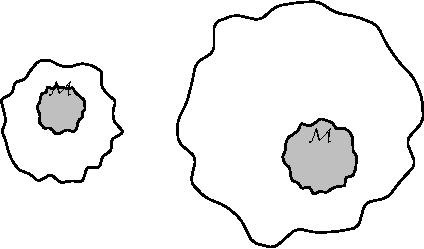
\includegraphics[width=0.6\textwidth]{U:/GitHub/Covariatesets/Diagrams/Identification.pdf}
\caption*{\footnotesize A model $\mathcal{M}$ is a set of structures that forms a proper subset of the class of all structures $\mathcal{S}$. Each structure in $\mathcal{M}$ generates a probability distribution in the class of all probability distributions (of observable variables) $\mathcal{P}$. Then the image $\mathcal{I}$ is the set of all probability distributions that are generated by structures in $\mathcal{M}$.}
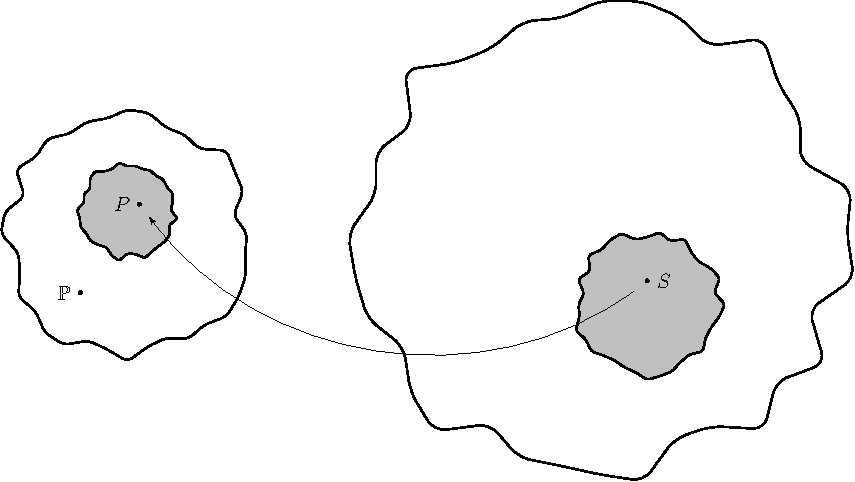
\includegraphics[width=0.6\textwidth]{U:/GitHub/Covariatesets/Diagrams/Observationalrestrictiveness.pdf}
\caption*{\footnotesize A structure $S$ is incompatible with data if it generates a probability distribution (of observable variables) $P$ that is distinct from a realised probability distribution $\mathbb{P}$. If all structures in $\mathcal{M}$ are incompatible with data then $\mathcal{M}$ is said to be observationally restrictive, and is falsified. This condition is equivalent to $\mathbb{P}\in\mathcal{P}\setminus\mathcal{I}$.}
\caption{Structures, models, probability distributions (of observable variables), and falsifiability.}
\label{fig:models}
\end{figure}
\clearpage
%==================================================%
\begin{figure}[p]
\centering
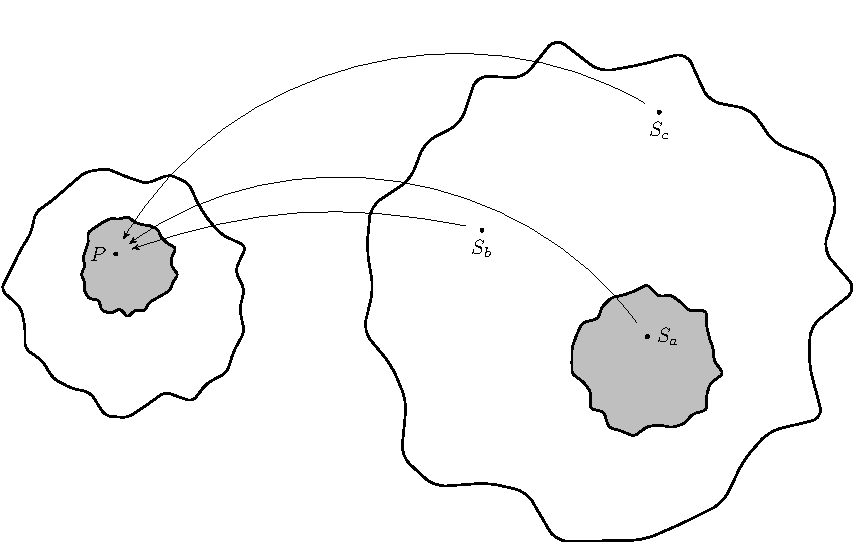
\includegraphics[width=0.6\textwidth]{U:/GitHub/Covariatesets/Diagrams/Pointidentification.pdf}
\caption*{\footnotesize A model $\mathcal{M}$ is said to identify a structure $S$ if the probability distribution (of observable variables) $P$ that is generated by $S$ is distinct from those generated by other structures in $\mathcal{M}$. The structures $S_a$, $S_b$ and $S_c$ are said to be observationally equivalent as they all generate $P$ but $S_b$ and $S_c$ are not admitted by $\mathcal{M}$. As $S_a$ is the only structure that is admitted by $\mathcal{M}$ and that generates $P$, $S_a$ is identified by $\mathcal{M}$. For completeness, $\mathcal{M}$ is said to be uniformly identifying if it identifies each structure that it admits.}
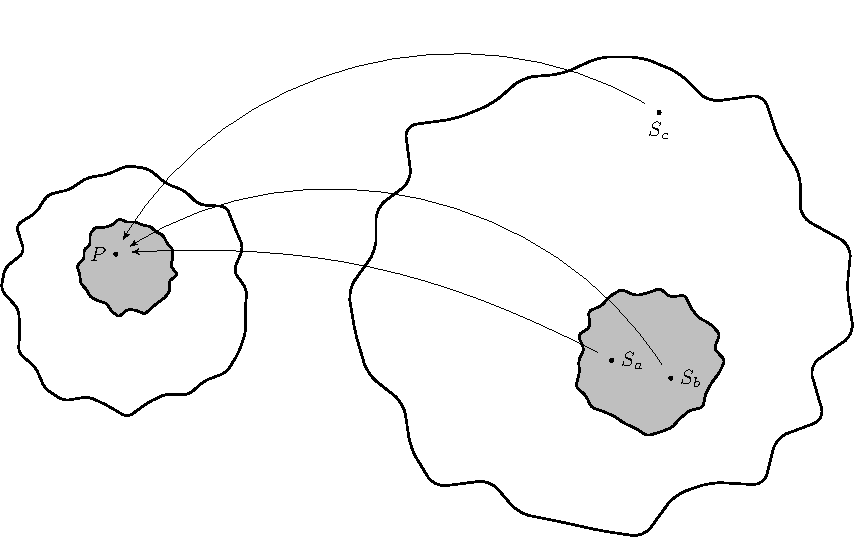
\includegraphics[width=0.6\textwidth]{U:/GitHub/Covariatesets/Diagrams/Setidentification.pdf}
\caption*{\footnotesize As $S_a$ and $S_b$ are observationally equivalent and are both admitted by $\mathcal{M}$ then $\mathcal{M}$ does not identify either $S_a$ or $S_b$. Nonetheless, as $\mathcal{M}$ restricts the set of observationally equivalent structures that generate $P$ to $S_a$ and $S_b$ then $\mathcal{M}$ partially identifies $S_a$ (and $S_b$ to within $\lbrace S_a,S_b\rbrace$).}
\caption{Identification and non-identification of a structure, and partial identification of a structure.}
\label{fig:identification}
\end{figure}
\clearpage
%==================================================%
\begin{figure}[p]
\centering
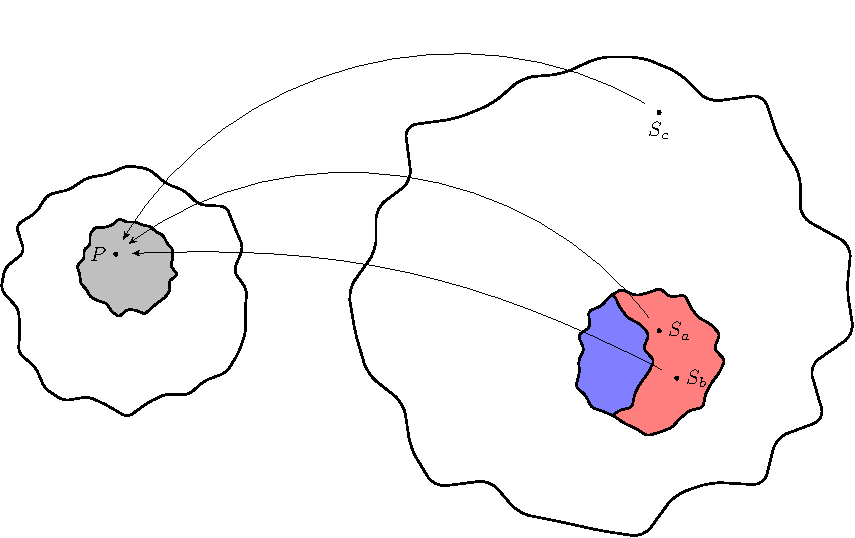
\includegraphics[width=0.6\textwidth]{U:/GitHub/Covariatesets/Diagrams/Characteristic.pdf}
\caption*{\footnotesize A structural characteristic $\chi$ is a function of a structure $S$. A model $\mathcal{M}$ can be partitioned such that structures in a partition deliver the same value for $\chi$. Structures in the red partition $\color{red}\mathcal{M}$ deliver the value $a$ for $\chi$, and structures in the blue partition $\color{blue}\mathcal{M}$ deliver the value $b$ for $\chi$. If $\chi$ is constant across all observationally equivalent structures that $\mathcal{M}$ admits then $\mathcal{M}$ is said to identify $\chi$. As $\chi(S_a)$ is equal to $\chi(S_b)$ (is equal to $a$) $\mathcal{M}$ identifies $\chi$.}
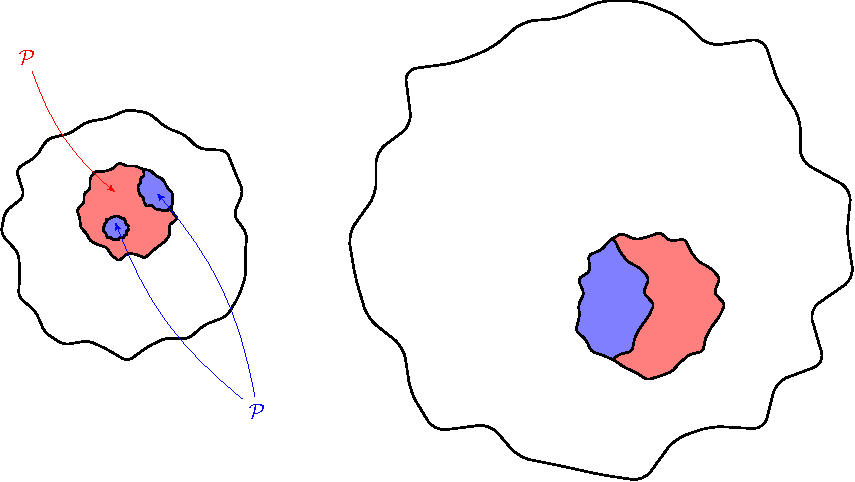
\includegraphics[width=0.6\textwidth]{U:/GitHub/Covariatesets/Diagrams/Uniform.pdf}
\caption*{\footnotesize If $\mathcal{M}$ identifies $\chi$ for all structures in $\mathcal{M}$ then $\mathcal{M}$ is said to uniformly identify $\chi$. The class of all probability distributions (of observable variables) is partitioned into the red partition $\color{red}\mathcal{P}$ and into the blue partition $\color{blue}\mathcal{P}$. Probability distributions in $\color{red}\mathcal{P}$ are generated by (potentially many) structures in $\color{red}\mathcal{M}$, and probability distributions in $\color{blue}\mathcal{P}$ are generated by (potentially many) structures in $\color{blue}\mathcal{M}$. It is important that the number of partitions in $\mathcal{M}$ and in $\mathcal{P}$ are equal, although that number can be countably infinite. In the context of Figure~\ref{fig:characteristics} $\mathcal{M}$ uniformly identifies $\chi$ since observationally equivalent structures that $\mathcal{M}$ admits are in the same colour of $\mathcal{M}$. More conveniently, whether $\mathcal{M}$ uniformly identifies $\chi$ can be determined by the existence of an identifying correspondence $G$, a functional. $\color{red}P$ is a probability distribution in $\color{red}\mathcal{P}$, and $\color{blue}P$ is a probability distribution in $\color{blue}\mathcal{P}$. Then $\mathcal{M}$ uniformly identifies $\chi$ if the value of $G(\color{red}P\color{black})$ is $a$ and if the value of $G(\color{blue}P\color{black})$ is $b$, holding for any such $\color{red}P$ and $\color{blue}P$. Notice that if $\mathcal{M}$ uniformly identifies all $\chi$ then $\mathcal{M}$ also uniformly identifies structures.}
\caption{The identification of structural characteristics, and identifying correspondences.}
\label{fig:characteristics}
\end{figure}
\clearpage
%==================================================%
\begin{figure}[p]
\centering
\caption*{\footnotesize A structural characteristic $\chi$ is a function of a structure $S$. A model $\mathcal{M}$ can be partitioned such that structures in a partition deliver the same value for $\chi$. Structures in the red partition $\color{red}\mathcal{M}$ deliver the value $a$ for $\chi$, structures in the blue partition $\color{blue}\mathcal{M}$ deliver the value $b$ for $\chi$, and structures in the yellow partition $\color{yellow}\mathcal{M}$ deliver the value $c$ for $\chi$. The class of all probability distributions (of observable variables) $\mathcal{P}$ is partitioned into the red partition $\color{red}\mathcal{P}$, into the blue partition $\color{blue}\mathcal{P}$, into the yellow partition $\color{yellow}\mathcal{P}$ and into the grey partition $\color{gray}\mathcal{P}$. Probability distributions in a colour of $\mathcal{P}$ are generated by (potentially many) structures in the same colour of $\mathcal{M}$; the exception is probability distributions in $\color{gray}\mathcal{P}$ which are generated by (potentially many) structures in $\color{red}\mathcal{M}$ and in $\color{yellow}\mathcal{M}$. $P$ is a probability distribution in $\mathcal{P}$ with probability distributions defined similarly for each colour in $\mathcal{P}$.}
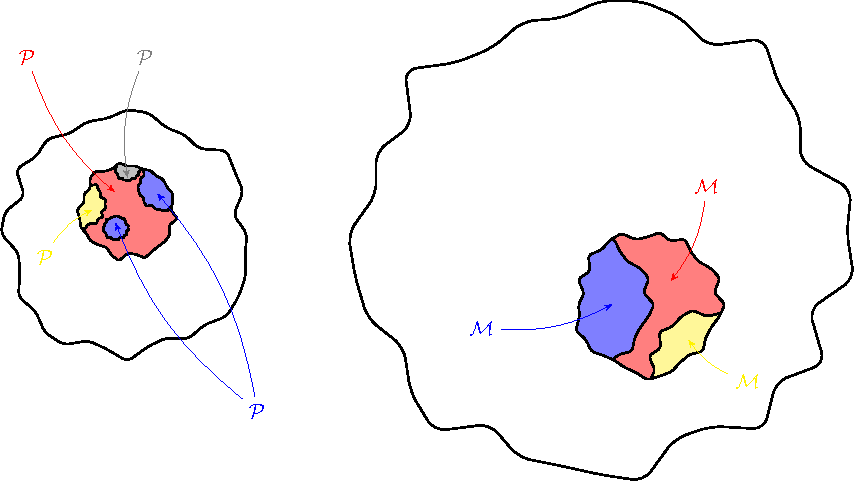
\includegraphics[width=0.6\textwidth]{U:/GitHub/Covariatesets/Diagrams/Partial.pdf}
\caption*{\footnotesize That probability distributions in $\color{gray}\mathcal{P}$ are generated by structures in $\color{red}\mathcal{M}$ and in $\color{yellow}\mathcal{M}$ creates a complication; the value of $\chi$ is not constant across observationally equivalent structures that $\mathcal{M}$ admits and that generate a probability distribution in $\color{gray}\mathcal{P}$. So $\mathcal{M}$ does not uniformly identify $\chi$. Consideration of the identifying correspondence $G$ determines that this corresponds to there being structures in $\mathcal{M}$ for which $G$ does not deliver the value of $\chi$ when applied to the probability distributions that these structures generate. Nonetheless, if $\mathcal{M}$ restricts the set of $\chi$ for any probability distribution in $\mathcal{P}$ then $\mathcal{M}$ does have some non-trivial identifying power for $\chi$. Then $\mathcal{M}$ is said to uniformly partially identify $\chi$ if $\mathcal{M}$ and $\mathcal{P}$ can each be partitioned into countably many disjoint subsets and that a probability distribution in a partition of $\mathcal{P}$ is not generated by a structure in at least one partition of $\mathcal{M}$, holding for any such partition of $\mathcal{P}$. In the context of Figure~\ref{fig:partials} $\color{red}\mathcal{M}$ identifies $\chi$ up to $\lbrace a,c\rbrace$, $\color{blue}\mathcal{M}$ identifies $\chi$ uniquely to $b$, and $\color{yellow}\mathcal{M}$ identifies $\chi$ up to $\lbrace a,c\rbrace$. Each partition of $\mathcal{P}$ includes probability distributions that are generated by structures in at least one partition of $\mathcal{M}$. Equivalently, if $G$ is permitted to be a multivalued functional (or one-to-many) then $\mathcal{M}$ uniformly partially identifies $\chi$ if $G$ exists and if $G(P)$ contains the set of $\chi$ that are delivered by structures that generate $P$, holding for all such $P$. A caveat must be applied here; $G$ cannot be trivial in the sense that it is constant across all such $P$. Clearly this definition of $G$ does not exclude the possibility that there is multiplicity of identifying correspondences that satisfy this property. Sharpness is a desirable property in such circumstances; a functional $G$ that can be shown to deliver smaller sets according to some well-defined distance measure across all possible $P$ (and that satisfies the properties above) should be preferred to any alternative identifying correspondence.}
\caption{Partial identification of a structural characteristic.}
\label{fig:partials}
\end{figure}
\clearpage
%==================================================%
\begin{figure}[p]
\centering
\begin{subfigure}{0.4\textwidth}
\centering
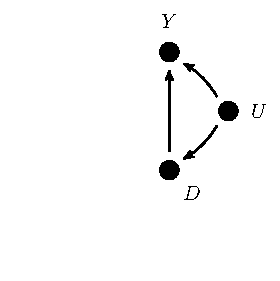
\includegraphics[width=0.75\textwidth]{U:/GitHub/Covariatesets/Diagrams/Indistinguishable1.pdf}
\label{fig:indistinguishable1}
\end{subfigure}
\begin{subfigure}{0.4\textwidth}
\centering
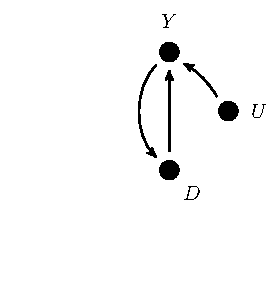
\includegraphics[width=0.75\textwidth]{U:/GitHub/Covariatesets/Diagrams/Indistinguishable2.pdf}
\label{fig:indistinguishable2}
\end{subfigure}
\caption*{\footnotesize The left- and right-hand panels show directed acyclic graphs that are able to represent the same probability distribution of $(Y,D)$. In the left-hand panel, $U$ causes $Y$ and $D$. The left-hand panel is a representation of selection in that particular values of $D$ are strongly associated with particular values of $Y$ independently of the causal effect of $D$. In the right-hand panel, $U$ causes $Y$ but has an indirect effect on $D$ through $Y$. The right-hand panel is a representation of simultaneity in that $Y$ is both a cause of and an effect of $D$. The equivalence between the two directed acyclic graphs is that $Y$ can always be written as $\xi(D,U)$ for $\xi : \mathcal{R}_D\times\mathcal{R}_U\rightarrow\mathcal{R}_Y$ (provided that the right-hand panel converges to an equilibrium).}
\begin{subfigure}{0.4\textwidth}
\centering
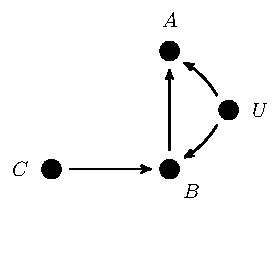
\includegraphics[width=0.75\textwidth]{U:/GitHub/Covariatesets/Diagrams/Exogenous1.pdf}
\label{fig:exogenous1}
\end{subfigure}
\begin{subfigure}{0.4\textwidth}
\centering
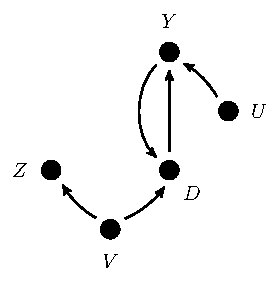
\includegraphics[width=0.75\textwidth]{U:/GitHub/Covariatesets/Diagrams/Exogenous2.pdf}
\label{fig:exogenous2}
\end{subfigure}
\caption*{\footnotesize To recover the causal effect of $D$ on $Y$, it is necessary that there exists an external and measurable factor that causes variation in $D$. This external and measurable factor is known as an instrumental variable. In the left-hand panel, $Z$ causes $D$. It is convenient to think of $Z$ as a switch that forces $D$ to take particular values. The difference between the value of $Y$ when $Z$ is $\mathtt{on}$ versus when $Z$ is $\mathtt{off}$ is the causal effect of $D$ on $Y$. In the right-hand panel, it is $V$ that causes $D$ ($V$ is unobservable). As $V$ causes $D$ and $Z$, it may be sufficient to look at $Z$ to measure exogenous variation in $D$ (although it is not always). As such, the causal effect of $D$ on $Y$ is recoverable using variation in $Z$. This is an important point about the nature of an instrumental variable; namely, that the relationship between $D$ and $Z$ need not be causal.}
\caption{A note on causality.}
\label{fig:causality}
\end{figure}
\clearpage
%==================================================%
\begin{figure}[p]
\centering
\caption*{\footnotesize Suppose that $\color{blue}\theta_n^u(z)\color{black}$ and $\color{red}\theta_n^u(z')\color{black}$ are estimates of upper bounds on $\mathbb{E}_n[Y(0)]$. Similarly, suppose that $\color{blue}\phi_n^u(z)\color{black}$ and $\color{red}\phi_n^u(z')\color{black}$ are one-sided $1-\alpha$ confidence regions for $\color{blue}\theta_n^u(z)\color{black}$ and $\color{red}\theta_n^u(z')\color{black}$. $\color{red}\phi_n^u(z')\color{black}>\color{blue}\phi_n^u(z')\color{black}$ if there is greater variation in the estimate of $\color{blue}\theta_n^u(z)\color{black}$ (if there are fewer observations of $z$ than $z'$, say).}
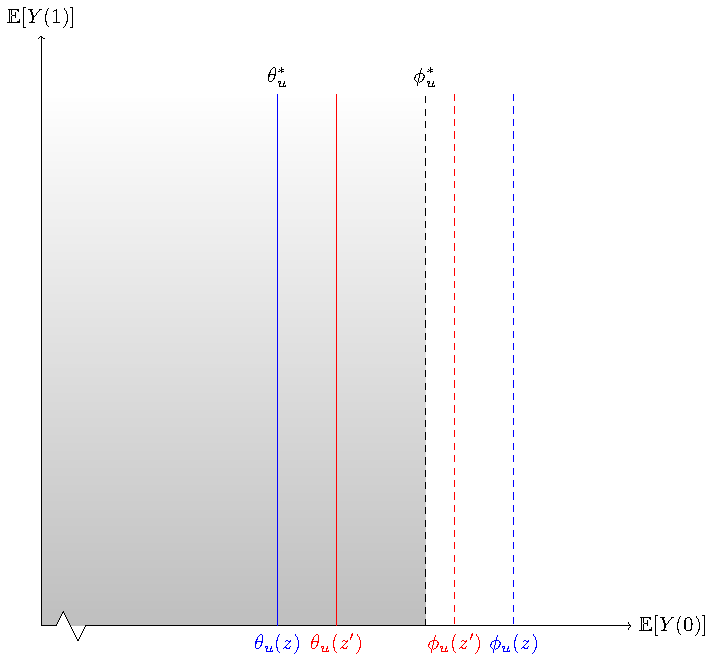
\includegraphics[width=0.75\textwidth]{U:/GitHub/Covariatesets/Diagrams/Confidence.pdf}
\caption*{\footnotesize As $\color{blue}\theta_n^u(z)\color{black}$ and $\color{red}\theta_n^u(z')\color{black}$ are both constraints on $\mathbb{E}_n[Y(0)]$, the minimum of these upper bounds must be binding. The minimum upper bound is written as $\theta^u_n$ and is $\color{blue}\theta_n^u(z)\color{black}$. The inferential problem is to determine $\phi_n^u$, which satisfies $\mathbb{P}(\mathbb{E}[Y(0)]>\phi_n^u)=\alpha$. A na{\"i}ve approach would be to look only at the one-sided $1-\alpha$ confidence region for $\color{blue}\theta_n^u(z)\color{black}$, which is $\color{blue}\phi_n^u(z)\color{black}$. This approach ignores variation in $\color{red}\theta_n^u(z')\color{black}$. An equally na{\"i}ve approach would be to simply add aggregate variation to $\color{blue}\theta_n^u(z)\color{black}$. In other words, to add the weighted average of $\color{blue}\phi_n^u(z)\color{black}-\color{blue}\theta_n^u(z)\color{black}$ and $\color{red}\phi_n^u(z')\color{black}-\color{red}\theta_n^u(z')\color{black}$ to $\color{blue}\theta_n^u(z)\color{black}$. This approach is standard but fails in this case because it does not account for the fact that $\color{blue}\theta_n^u(z)\color{black}<\color{red}\theta_n^u(z')\color{black}$. Inference must account for the fact that upward variation in $\color{red}\theta_n^u(z')\color{black}$ does not matter so long as $\color{blue}\theta_n^u(z)\color{black}<\color{red}\theta_n^u(z')\color{black}$; equivalently, that $\color{red}\theta_n^u(z')\color{black}$ is a one-sided $1-\gamma$ confidence region for $\color{blue}\theta_n^u(z)\color{black}$ for $\gamma>\alpha$. \cite{cHlr13} solves the inferential problem by adjusting the critical value that is associated with the one-sided $1-\alpha$-confidence region. That is, \cite{cHlr13} adjusts $k$ such that $k$ that solves $\mathbb{P}(\mathbb{E}[Y(0)]>\color{blue}\theta_n^u(z)\color{black}+k\sigma)=\alpha$. The solution for $k$ yields $\phi_n^u$ with the one-sided $1-\alpha$ confidence region for $\theta_n^u$ given by the grey area. The distribution of $\theta_n^u$ over repeated samples is non-standard in this case and the bootstrap is not necessarily consistent \citep{bU10}.} 
\caption{A note on the inferential problem.}
\label{fig:confidence}
\end{figure}
\clearpage
%==================================================%
\begin{figure}[p]
\centering
\caption*{\footnotesize Suppose that the estimate of the identified set of $(\mathbb{E}[Y(0)],\mathbb{E}[Y(1)])$ is given by the blue rectangle, and that the $1-\alpha$-confidence region for this set is the union of the blue rectangle and the red polygon.}
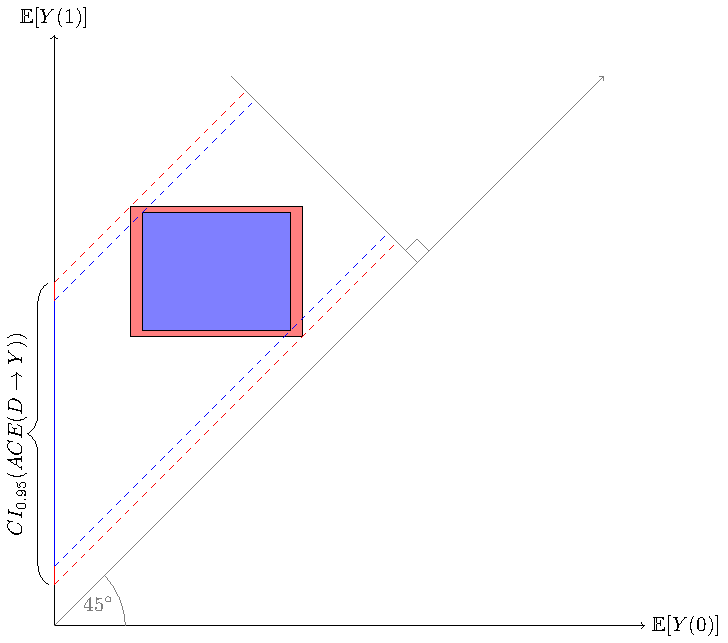
\includegraphics[width=0.75\textwidth]{U:/GitHub/Covariatesets/Diagrams/ACE.pdf}
\caption*{\footnotesize It is possible to recover $ACE(D\rightarrow Y)$ from the plot. First, note that $ACE(D\rightarrow Y)$ is increasing in the $y$-direction and is decreasing in the $x$-direction. Second, note that $ACE(D\rightarrow Y)$ is constant along any line with unit gradient. Third, note that the value of $ACE(D\rightarrow Y)$ along any line with unit gradient is dependent upon the value of the intercept of this line. Fourth, note that a projection from the normal of a line with unit gradient is a line that has unit gradient. For example, the blue dashed line is a projection from the normal of the $45^\circ$ line; notice that the blue dashed line is parallel to the $45^\circ$ line. Fifth, note that any projection from the normal of the $45^\circ$ line that passes through the blue rectangle is an admissible value of $(\mathbb{E}[Y(0)],\mathbb{E}[Y(1)])$; equivalently, that any projection from the normal of the $45^\circ$ line that passes through the union of the blue rectangle and the red polygon is in the $1-\alpha$ confidence region of $(\mathbb{E}[Y(0)],\mathbb{E}[Y(1)])$. Together these five facts suggest that the estimate of the identified set of $ACE(D\rightarrow Y)$ and its $1-\alpha$ confidence region can be recovered from the projection from the normal of the $45^\circ$ line onto the $y$-axis. This method gives a geometric interpretation to $ACE(D\rightarrow Y)$.}
\caption{A note on recovering the average causal effect.}
\label{fig:ace}
\end{figure}
\clearpage
%==================================================%
\begin{figure}[p]
\centering
\caption*{\footnotesize The plot shows how the estimate of the identified set of $ACE_n(D\rightarrow Y)$ changes as $\mathcal{R}_Z$ is varied. Each value on the $y$-axis corresponds to a different specification. In each specification, $\mathcal{R}_Z$ is varied and the estimate of the identified set of $ACE_n(D\rightarrow Y)$ is calculated. See Table~\ref{tbl:acesame} and Table~\ref{tbl:acemult} for the definition of $\mathcal{R}_Z$ in each specification (the column headed No. states the specification number in each table, and the column headed $\mathcal{R}_Z$ states the events that form the points of support for $Z$). The plot is a graphical representation of Table~\ref{tbl:acesame} and Table~\ref{tbl:acemult}. Blue regions represent the estimate of the identified set of $ACE_n(D\rightarrow Y)$, and the union of blue and red regions represent $0.950$ confidence regions for $ACE_n(D\rightarrow Y)$.}
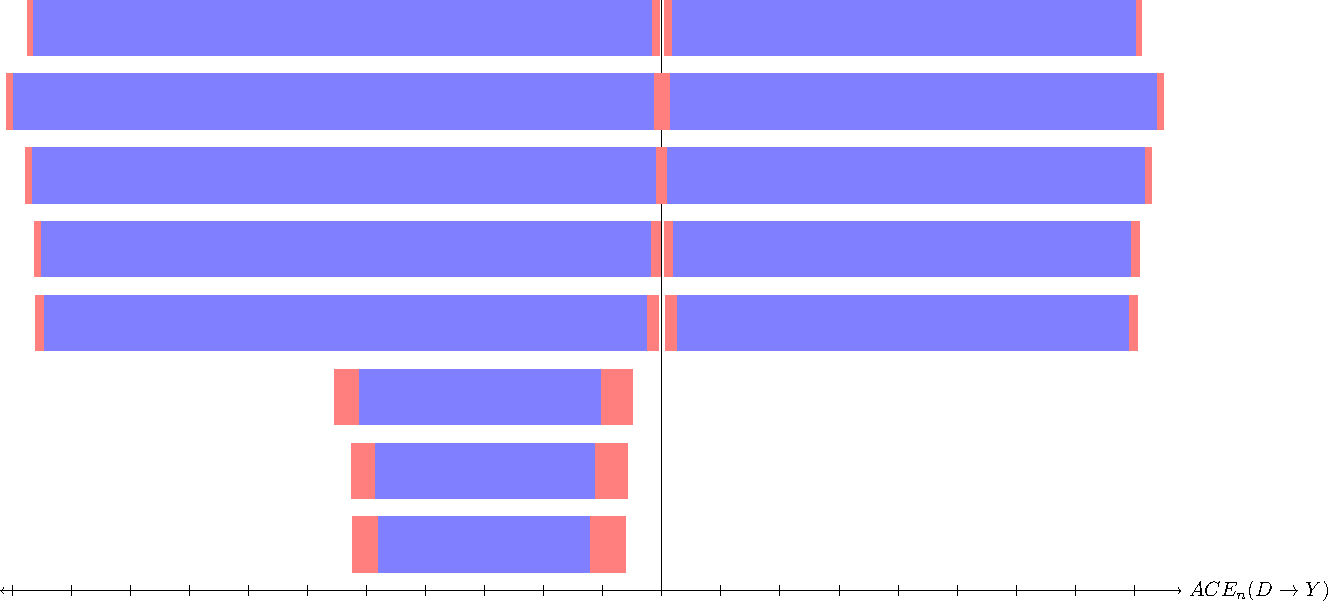
\includegraphics[width=0.75\textwidth]{U:/GitHub/Covariatesets/Coding/tikzDevice/Instruments.pdf}
\caption*{\footnotesize In Specification 1 through Specification 5, information relating to the incidence of a multiple second birth is ignored. The estimate of the identified sets of values of $ACE_n(D\rightarrow Y)$ in these specifications are large and disconnected, which suggests that child gender is weakly associated with the number of children in a household. In other words, that child gender is a weak instrumental variable. Child gender is, by itself, insufficient to determine the sign of the average causal effect of the number of children in a household on a mother's employment. Specification 2 and Specification 3 are unable to rule out a null effect at the $0.950$ significance level (the central red regions overlap at zero). In Specification 6 through Specification 7, information relating to the incidence of a multiple second birth is incorporated. The sign of the average causal effect of the number of children in a household on a mother's employment is negative, and significant. The length of the estimate of the identified set of $ACE_n(D\rightarrow Y)$ is decreasing as more information is incorporated, as is the $0.950$ confidence region for $ACE_n(D\rightarrow Y)$.}
\caption{Admissible sets of values of $ACE_n(D\rightarrow Y)$ and $\mathcal{R}_Z$.}
\label{fig:experiments}
\end{figure}
\clearpage
%==================================================%
\begin{figure}[p]
\centering
\caption*{\footnotesize The plot shows the estimate of the identified set of $(\mathbb{E}_n[Y(0)],\mathbb{E}_n[Y(1)])$ when $\mathcal{R}_Z$ is formed of the events $\text{Male-Male}\cup\text{Female-Female}$ and $\text{Male-Female}\cup\text{Female-Male}$. This is Specification 1 in Table~\ref{tbl:setssame}. Blue regions represent the estimate of the identified set of $(\mathbb{E}_n[Y(0)],\mathbb{E}_n[Y(1)])$, and the union of blue and red regions represent $0.950$ confidence regions for $(\mathbb{E}_n[Y(0)],\mathbb{E}_n[Y(1)])$. The confidence regions that are shown in the plot are different to those that are reported in Table~\ref{tbl:setssame}. The distinction arises since Table~\ref{tbl:setssame} reports $0.950$ confidence regions for $\mathbb{E}_n[Y(0)]$ and for $\mathbb{E}_n[Y(1)]$ whereas the plot shows the $0.950$ confidence region for $(\mathbb{E}_n[Y(0)],\mathbb{E}_n[Y(1)])$.}
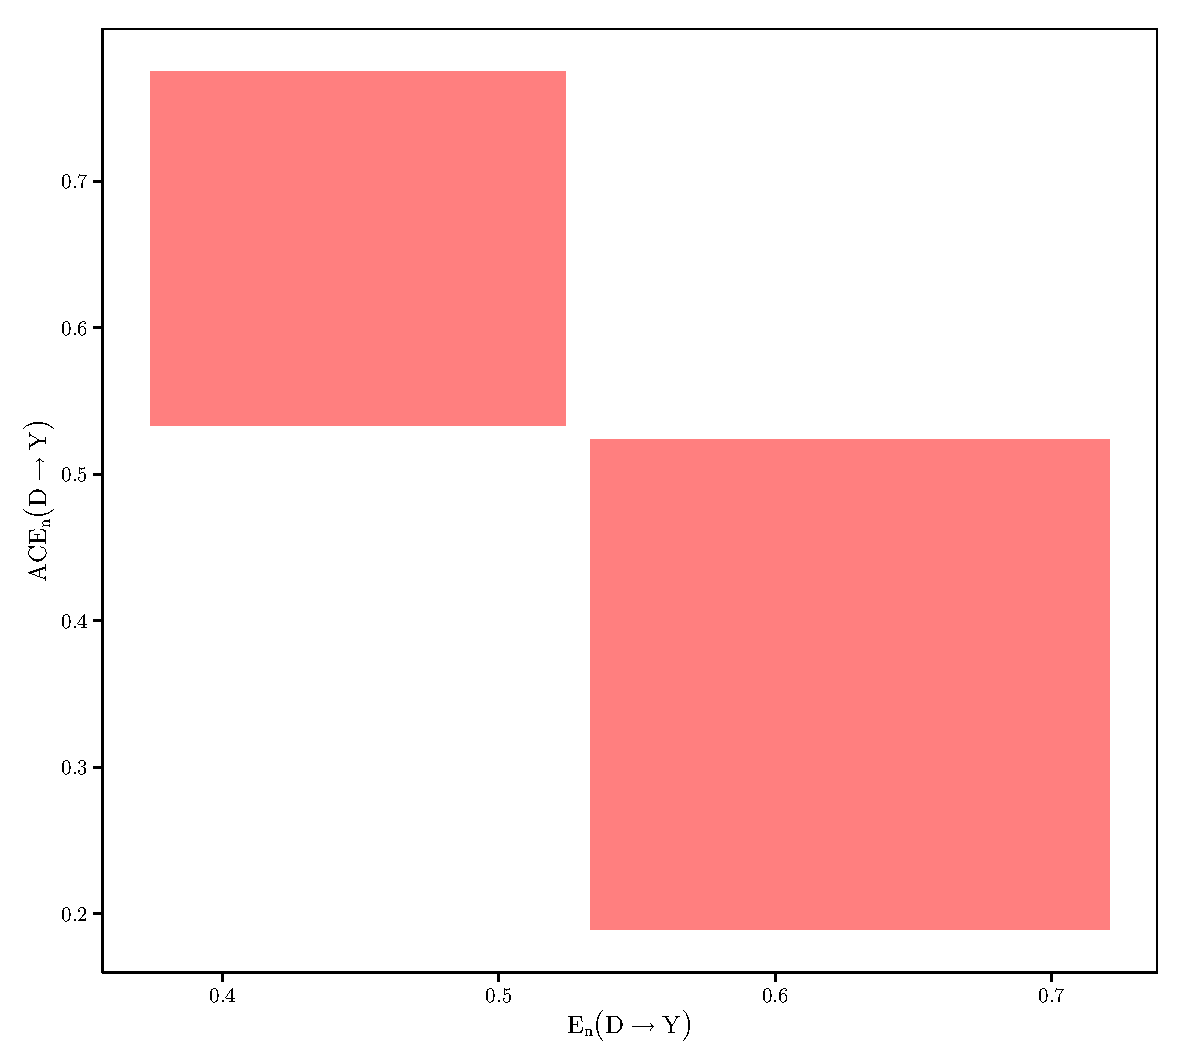
\includegraphics[width=0.75\textwidth]{U:/GitHub/Covariatesets/Coding/tikzDevice/Samesex.pdf}
\caption{}
\label{fig:samesex}
\end{figure}
\clearpage
%==================================================%
\begin{figure}[p]
\centering
\begin{subfigure}{0.8\textwidth}
\caption{The plot shows the estimate of the identified set of $(\mathbb{E}_n[Y(0)],\mathbb{E}_n[Y(1)])$ when $\mathcal{R}_Z$ is formed of the events $\text{Multiple birth}$, $\text{Single birth}\cap(\text{Male-Male}\cup\text{Female-Female})$ and $\text{Single birth}\cap(\text{Male-Female}\cup\text{Male-Female})$. This is Specification 6 in Table~\ref{tbl:setsmult}. Blue regions represent the estimate of the identified set of $(\mathbb{E}_n[Y(0)],\mathbb{E}_n[Y(1)])$, and the union of blue and red regions represent $0.950$ confidence regions for $(\mathbb{E}_n[Y(0)],\mathbb{E}_n[Y(1)])$. The confidence regions that are shown in the plot are different to those that are reported in Table~\ref{tbl:setsmult}. The distinction arises since Table~\ref{tbl:setsmult} reports $0.950$ confidence regions for $\mathbb{E}_n[Y(0)]$ and for $\mathbb{E}_n[Y(1)]$ whereas the plot shows the $0.950$ confidence region for $(\mathbb{E}_n[Y(0)],\mathbb{E}_n[Y(1)])$.}
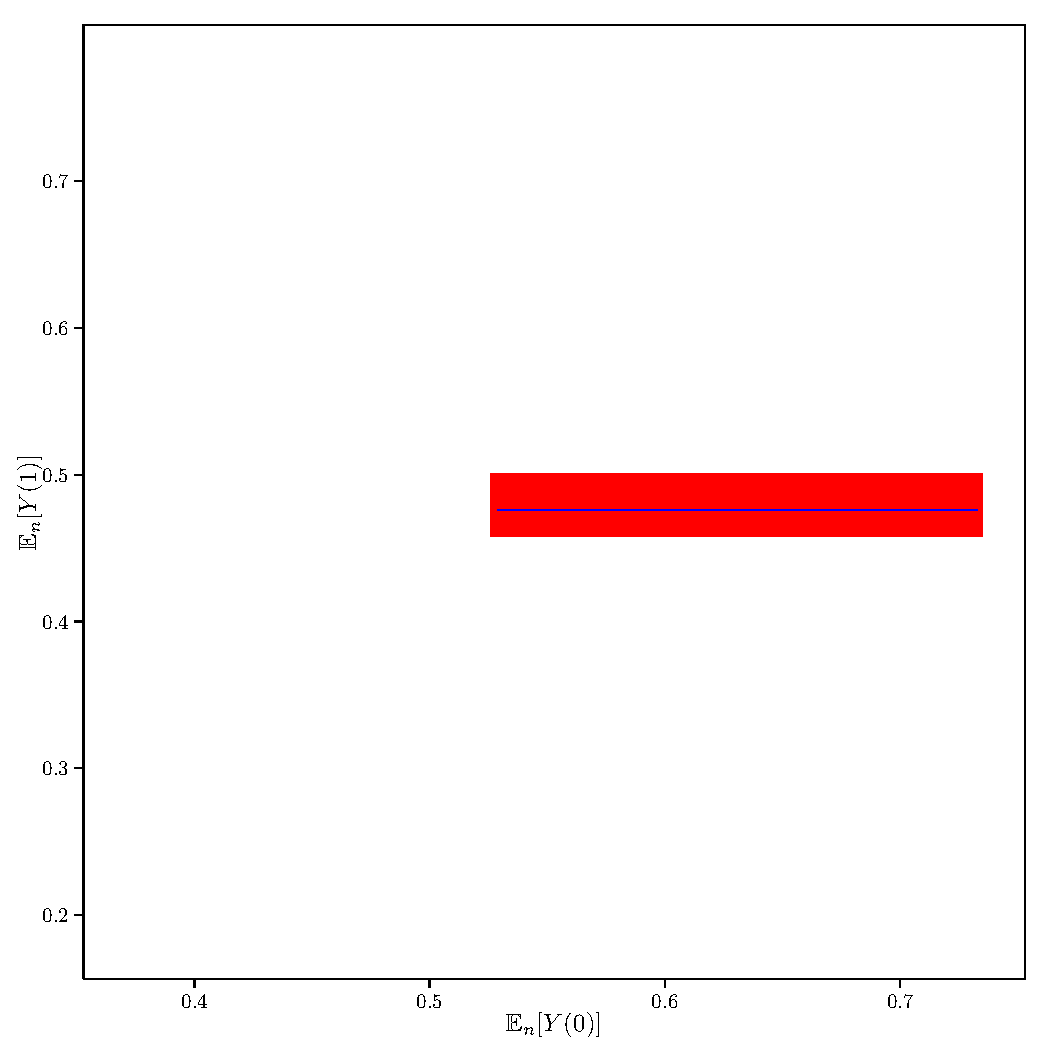
\includegraphics[width=\textwidth]{U:/GitHub/Covariatesets/Coding/tikzDevice/Multiple.pdf}
\caption{}
\end{subfigure}
\caption{}
\label{fig:multiple}
\end{figure}
%==================================================%
\begin{figure}[p]
\centering
\begin{subfigure}{0.8\textwidth}
\caption{The plot shows the estimate of the identified set of $(\mathbb{E}_n[Y(0)],\mathbb{E}_n[Y(1)])$ when $\mathcal{R}_Z$ is formed of the events $\text{Multiple birth}$, $\text{Single birth}\cap\text{Male-Male}$, $\text{Single birth}\cap\text{Female-Female}$, $\text{Single birth}\cap\text{Male-Female}$ and $\text{Single birth}\cap\text{Female-Male}$. This is Specification 8 in Table~\ref{tbl:setsmult}. Blue regions represent the estimate of the identified set of $(\mathbb{E}_n[Y(0)],\mathbb{E}_n[Y(1)])$, and the union of blue and red regions represent $0.950$ confidence regions for $(\mathbb{E}_n[Y(0)],\mathbb{E}_n[Y(1)])$. The confidence regions that are shown in the plot are different to those that are reported in Table~\ref{tbl:setsmult}. The distinction arises since Table~\ref{tbl:setsmult} reports $0.950$ confidence regions for $\mathbb{E}_n[Y(0)]$ and for $\mathbb{E}_n[Y(1)]$ whereas the plot shows the $0.950$ confidence region for $(\mathbb{E}_n[Y(0)],\mathbb{E}_n[Y(1)])$.}
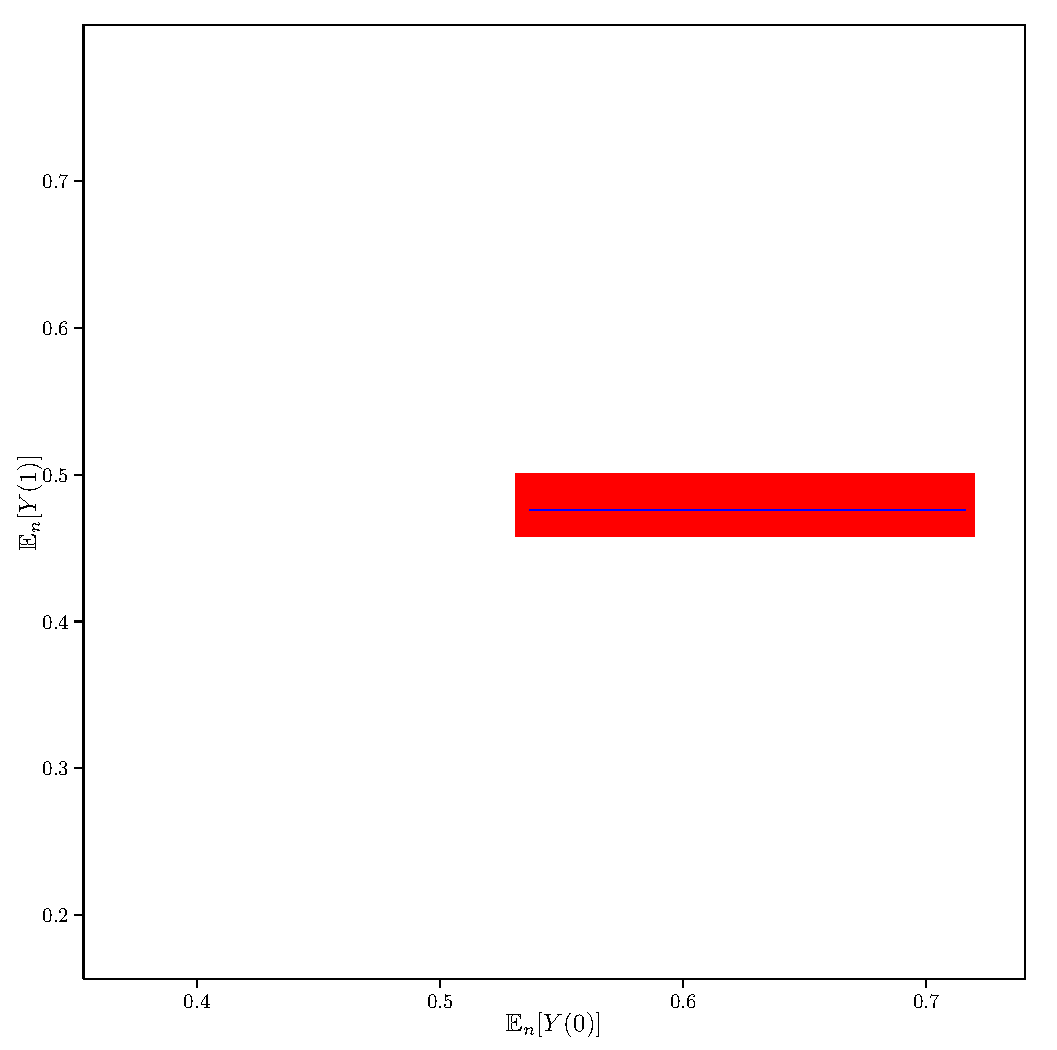
\includegraphics[width=\textwidth]{U:/GitHub/Covariatesets/Coding/tikzDevice/Allin.pdf}
\caption{}
\end{subfigure}
\caption{}
\label{fig:allin}
\end{figure}
%==================================================%
\begin{figure}[p]
\centering
\caption*{\footnotesize The goal of the identification analysis is to determine the location of $r(0)$ and of $r(1)$. The analysis is confounded by the fact that it is not known whether $r(0)>r(1)$, $r(0)<r(1)$ or $r(0)=r(1)$. The order of the collection of $r(d)$ is crucial since it is the order that determines the value of $\mathcal{A}_r$ and of $\mathcal{B}_r$. Suppose that $r(0)<r(1)$. What can be determined about the location of $p(0)$ from observable variables alone? Any economic agent that is characterised by $\color{blue}Y=0\cap D=0\color{black}$ must also be characterised by $u$ somewhere in the blue dashed interval. Similarly, any economic agent that is characterised by $\color{red}Y=0\cap D=1\color{black}$ must also be characterised by $u$ somewhere in the red dashed interval. The location of $r(0)$ is confounded since it is not known what proportion of $\color{red}Y=0\cap D=1\color{black}$ are located in $[0,r(0)]$ (the left partition of the red dashed interval), and what proportion of $\color{red}Y=0\cap D=1\color{black}$ are located in $(r(0),r(1)]$ (the right partition of the red dashed interval). A lower bound on the location of $r(0)$ is then that all economic agents that are are characterised by $\color{red}Y=0\cap D=1\color{black}$ are located in $(r(0),r(1)]$. The measure of economic agents that are located in $[0,r(0)]$ in this case is then $\mathbb{P}(Y=0,D=\color{blue}0\color{black})$. An upper bound on the location of $r(0)$ is then that all economic agents that are are characterised by $\color{red}Y=0\cap D=1\color{black}$ are located in $[0,r(0)]$. The measure of economic agents that are located in $[0,r(0)]$ in this case is then $\mathbb{P}(Y=0,D=\color{blue}0\color{black}\cup\color{red}1\color{black})$. For this order, $\mathcal{A}_r(0)=\lbrace 0\rbrace$ and $\mathcal{B}_r(0)=\lbrace 0,1\rbrace$.}
\vspace{20pt}
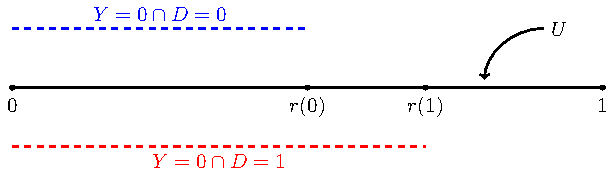
\includegraphics[width=0.75\textwidth]{U:/GitHub/Covariatesets/Diagrams/Timeline.pdf}
\vspace{20pt}
\caption*{\footnotesize Note that economic agents that are located in $[0,r(0)]$ are characterised by $Y(0)=0$ and $Y(1)=0$. In contrast, economic agents that are located in $(r(0),r(1)]$ are characterised by $Y(0)=1$ and $Y(1)=0$. The problem of determining the measure of economic agents that are characterised by each pair $(Y(0),Y(1))$ is then equivalent to locating $r(0)$ and $r(1)$. This point validates consideration of level sets of $U$.}
\caption{A note on partial identification.}
\label{fig:timeline}
\end{figure}
\clearpage
%==================================================%
%% Tables
%==================================================%
\renewcommand{\baselinestretch}{1}
\begin{sidewaystable}[p]
\centering
\caption{$\mathcal{R}_Z$ and estimate of the identified sets of values of $\mathbb{E}_n[Y(d)]$.}
\begin{tabular}{lclcrcrcrcr}
\toprule
&	& &	& \multicolumn{7}{c}{Bound} \\
\cmidrule(r){4-11}	
No. & &	$\mathcal{R}_Z$	&	&	$\mathbb{E}_n^-[Y(0)]$	&	&	$\mathbb{E}_n^-[Y(1)]$	&	&	$\mathbb{E}_n^+[Y(0)]$	&	&	$\mathbb{E}_n^+[Y(1)]$\\
\midrule
& &\phantom{$\text{Male-Female}\cup\text{Female-Male}\cup\text{Female-Female}$}\\
%1	
1& & $\text{Male-Male}\cup\text{Female-Female}$	&	&	$[0.533,0.721]$	&	&	$[0.189,0.524]$	&	&	$[0.374,0.524]$	&	&	$[0.533,0.775]$
\\
& &$\text{Male-Female}\cup\text{Female-Male}$	&	&	\color{blue}$[0.530,0.723]$	&	&	\color{blue}$[0.187,0.527]$	&	&	\color{blue}$[0.371,0.527]$	&	&	\color{blue}$[0.530,0.777]$\\
\\
%2
2 & &$\text{Male-Male}$	&	&	$[0.530,0.731]$	&	&	$[0.182,0.523]$	&	&	$[0.359,0.523]$	&	&	$[0.530,0.778]$
\\
& &$\text{Male-Female}\cup\text{Female-Male}\cup\text{Female-Female}$	&	&	\color{blue}$[0.528,0.733]$	&	&	\color{blue}$[0.179,0.527]$	&	&	\color{blue}$[0.357,0.527]$	&	&	\color{blue}$[0.528,0.781]$\\
\\
%3
3 & &$\text{Female-Female}$	&	&	$[0.529,0.729]$	&	&	$[0.196,0.524]$	&	&	$[0.362,0.524]$	&	&	$[0.529,0.771]$
\\
& &$\text{Male-Male}\cup\text{Male-Female}\cup\text{Female-Male}$	& &\color{blue}$[0.527,0.731]$	&	&	\color{blue}$[0.193,0.529]$	&	&	\color{blue}$[0.360,0.529]$	&	&	\color{blue}$[0.527,0.774]$\\	
\\
%4
4 & &$\text{Male-Male}$&	&	$[0.533,0.721]$	&	&	$[0.196,0.523]$	&	&	$[0.374,0.523]$	&	&	$[0.533,0.771]$
\\
& &$\text{Female-Female}$ & &\color{blue}$[0.530,0.723]$	&	&	\color{blue}$[0.192,0.528]$	&	&	\color{blue}$[0.371,0.528]$	&	&	\color{blue}$[0.530,0.775]$\\
& &$\text{Male-Female}\cup\text{Female-Male}$\\	
\\
%5
5 & &$\text{Male-Male}$&	&	$[0.536,0.718]$	&	&	$[0.196,0.523]$	&	&	$[0.376,0.523]$	&	&	$[0.536,0.771]$
\\
& &$\text{Female-Female}$& &\color{blue}$[0.531,0.722]$	&	&	\color{blue}$[0.193,0.528]$	&	&	\color{blue}$[0.372,0.528]$	&	&	\color{blue}$[0.531,0.775]$\\
& &$\text{Male-Female}$ \\
& &$\text{Female-Male}$\\	
	\\
\bottomrule
\end{tabular}
\vspace{10pt}
\renewcommand{\baselinestretch}{1.5}
\caption*{\scriptsize The column headed No. states the specification number. The column headed $\mathcal{R}_Z$ states the events that form the points of support of $Z$. For example, in Specification 1 $Z$ is a random variable that takes the value $z$ when the event $\text{Male-Male}\cup\text{Female-Female}$ occurs and the value $z'$ when this does not occur. The event $Male-Female$ is the event that the oldest two children in a household are male and female, respectively. The columns headed Bound are the estimate of the identified set of $\mathbb{E}_n[Y(D)]$. A superscript $-$ is written when the bounds are conditional on $\mathbb{E}_n[Y(0)]\geq\mathbb{E}_n[Y(1)]$, and a superscript $+$ is written when the bounds are conditional on $\mathbb{E}_n[Y(0)]\leq\mathbb{E}_n[Y(1)]$. $0.950$ confidence regions for $\mathbb{E}_n[Y(D)]$ are in blue and are constructed from one-sided $0.975$ confidence regions for the lower bound and the upper bound.}
\label{tbl:setssame}
\end{sidewaystable}
\clearpage
%==================================================%
\renewcommand{\baselinestretch}{1}
\begin{sidewaystable}[p]
\centering
\caption{$\mathcal{R}_Z$ and estimate of the identified sets of values of $\mathbb{E}_n[Y(d)]$.}
\begin{tabular}{lclcrcr}
\toprule
&	&  & &\multicolumn{3}{c}{Bound} \\
\cmidrule(r){4-7}	
No. & &	$\mathcal{R}_Z$	&	&	$\mathbb{E}_n^-[Y(0)]$	&	&	$\mathbb{E}_n^-[Y(1)]$\\
\midrule
& &\phantom{$\text{Male-Female}\cup\text{Female-Male}\cup\text{Female-Female}$}\\
%6
6& &$\text{Multiple birth}$&	&	$[0.529,0.733]$	&	&	$0.476$\\
& &$\text{Single birth}$& &\color{blue}$[0.526,0.734]$	&	&	\color{blue}$[0.460,0.498]$\\
\\
%7
7& &$\text{Multiple birth}$&	&	$[0.534,0.718]$	&	&	$0.476$\\
& &$\text{Single birth}\cap(\text{Male-Male}\cup\text{Female-Female})$& &\color{blue}$[0.530,0.721]$	&	&	\color{blue}$[0.460,0.498]$\\
& &$\text{Single birth}\cap(\text{Male-Female}\cup\text{Female-Male})$\\
\\
%8
8& &$\text{Multiple birth}$&	&	$[0.537,0.716]$	&	&	$0.476$\\
& &$\text{Single birth}\cap\text{Male-Male}$& &\color{blue}$[0.532,0.720]$	&	&	\color{blue}$[0.460,0.498]$\\
& &$\text{Single birth}\cap\text{Female-Female}$\\
& &$\text{Single birth}\cap\text{Male-Female}$ \\
& &$\text{Single birth}\cap\text{Female-Male}$\\
	\\
\bottomrule
\end{tabular}
\vspace{10pt}
\renewcommand{\baselinestretch}{1.5}
\caption*{\scriptsize The column headed No. states the specification number. The column headed $\mathcal{R}_Z$ states the events that form the points of support of $Z$. For example, in Specification 1 $Z$ is a random variable that takes the value $z$ when the event $\text{Male-Male}\cup\text{Female-Female}$ occurs and the value $z'$ when this does not occur. The event $Male-Female$ is the event that the oldest two children in a household are male and female, respectively. The columns headed Bound are the estimate of the identified set of $\mathbb{E}_n[Y(D)]$. A superscript $-$ is written when the bounds are conditional on $\mathbb{E}_n[Y(0)]\geq\mathbb{E}_n[Y(1)]$, and a superscript $+$ is written when the bounds are conditional on $\mathbb{E}_n[Y(0)]\leq\mathbb{E}_n[Y(1)]$. $0.950$ confidence regions for $\mathbb{E}_n[Y(D)]$ are in blue and are constructed from one-sided $0.975$ confidence regions for the lower bound and the upper bound.}
\label{tbl:setsmult}
\end{sidewaystable}
\clearpage
%==================================================%
\renewcommand{\baselinestretch}{1}
\begin{sidewaystable}[p]
\centering
\caption{$\mathcal{R}_Z$ and estimate of the identified sets of values of $ACE_n(D\rightarrow Y)$.}
\begin{tabular}{lclcrcr}
\toprule
&	&  & &\multicolumn{3}{c}{Bound} \\
\cmidrule(r){4-7}	
No.& &	$\mathcal{R}_Z$	&	&	$ACE_n^-(D\rightarrow Y)$	&	&	$ACE_n^+(D\rightarrow Y)$\\
\midrule
& &\phantom{$\text{Male-Female}\cup\text{Female-Male}\cup\text{Female-Female}$}\\
%1	
1& &$\text{Male-Male}\cup\text{Female-Female}$	&	&	$[-0.532,-0.009]$	&	&	$[0.009,0.401]$	\\
& &$\text{Male-Female}\cup\text{Female-Male}$	&	&	\color{blue}$[-0.537,-0.002]$	&	&	\color{blue}$[0.002,0.406]$	\\
\\
%2
2& &$\text{Male-Male}$	&	&	$[-0.549,-0.007]$	&	&	$[0.007,0.419]$	\\
& &$\text{Male-Female}\cup\text{Female-Male}\cup\text{Female-Female}$	&	&	\color{blue}$[-0.555,0.001]$	&	&	\color{blue}$[-0.001,0.425]$\\
\\
%3
3& &$\text{Female-Female}$	&	&	$[-0.533,-0.005]$	&	&	$[0.005,0.409]$	\\
& &$\text{Male-Male}\cup\text{Male-Female}\cup\text{Female-Male}$	& &\color{blue}$[-0.539,0.003]$	&	&	\color{blue}$[-0.003,0.415]$\\	
\\
%4
4& &$\text{Male-Male}$&	&	$[-0.525,-0.010]$	&	&	$[0.010,0.397]$	\\
& &$\text{Female-Female}$ & &\color{blue}$[-0.531,-0.001]$	&	&	\color{blue}$[0.002,0.404]$\\
& &$\text{Male-Female}\cup\text{Female-Male}$\\	
\\
%5
5& &$\text{Male-Male}$&	&	$[-0.523,-0.013]$	&	&	$[0.013,0.395]$	\\
& &$\text{Female-Female}$& &\color{blue}$[-0.530,-0.003]$	&	&	\color{blue}$[0.003,0.403]$	\\
& &$\text{Male-Female}$ \\
& &$\text{Female-Male}$\\	
	\\
\bottomrule
\end{tabular}
\vspace{10pt}
\renewcommand{\baselinestretch}{1.5}
\caption*{\scriptsize The column headed No. states the specification number. The column headed $\mathcal{R}_Z$ states the events that form the points of support of $Z$. For example, in Specification 1 $Z$ is a random variable that takes the value $z$ when the event $\text{Male-Male}\cup\text{Female-Female}$ occurs and the value $z'$ when this does not occur. The event $Male-Female$ is the event that the oldest two children in a household are male and female, respectively. The columns headed Bound are the estimate of the identified set of $ACE_n(D\rightarrow Y)$. A superscript $-$ is written when the bounds are conditional on $ACE_n(D\rightarrow Y)\leq 0$, and a superscript $+$ is written when the bounds are conditional on $ACE_n(D\rightarrow Y)\geq 0$. $0.950$ confidence regions for $ACE_n(D\rightarrow Y)$ are in blue and are constructed from one-sided $0.975$ confidence regions for the lower bound and the upper bound.}
\label{tbl:acesame}
\end{sidewaystable}
\clearpage
%==================================================%
\renewcommand{\baselinestretch}{1}
\begin{sidewaystable}[p]
\centering
\caption{$\mathcal{R}_Z$ and estimate of the identified sets of values of $ACE_n(D\rightarrow Y)$.}
\begin{tabular}{lclcr}
\toprule
&	& & & \multicolumn{1}{c}{Bound} \\
\cmidrule(r){5-5}	
No.& &	$\mathcal{R}_Z$	&	&	$ACE_n^-(D\rightarrow Y)$\\
\midrule
& &\phantom{$\text{Male-Female}\cup\text{Female-Male}\cup\text{Female-Female}$}\\
%6
6& &$\text{Multiple birth}$&	&	$[-0.256,-0.052]$\\
& &$\text{Single birth}$& &\color{blue}$[-0.277,-0.025]$	\\
\\
%7
7& &$\text{Multiple birth}$&	&	$[-0.242,-0.057]$	\\
& &$\text{Single birth}\cap(\text{Male-Male}\cup\text{Female-Female})$& &\color{blue}$[-0.263,-0.029]$\\
& &$\text{Single birth}\cap(\text{Male-Female}\cup\text{Female-Male})$\\
\\
%8
8& &$\text{Multiple birth}$&	&	$[-0.240,-0.061]$	\\
& &$\text{Single birth}\cap\text{Male-Male}$& &\color{blue}$[-0.262,-0.031]$	\\
& &$\text{Single birth}\cap\text{Female-Female}$\\
& &$\text{Single birth}\cap\text{Male-Female}$ \\
& &$\text{Single birth}\cap\text{Female-Male}$\\
	\\
\bottomrule
\end{tabular}
\vspace{10pt}
\renewcommand{\baselinestretch}{1.5}
\caption*{\scriptsize The column headed No. states the specification number. The column headed $\mathcal{R}_Z$ states the events that form the points of support of $Z$. For example, in Specification 1 $Z$ is a random variable that takes the value $z$ when the event $\text{Male-Male}\cup\text{Female-Female}$ occurs and the value $z'$ when this does not occur. The event $Male-Female$ is the event that the oldest two children in a household are male and female, respectively. The columns headed Bound are the estimate of the identified set of $ACE_n(D\rightarrow Y)$. A superscript $-$ is written when the bounds are conditional on $ACE_n(D\rightarrow Y)\leq 0$, and a superscript $+$ is written when the bounds are conditional on $ACE_n(D\rightarrow Y)\geq 0$. $0.950$ confidence regions for $ACE_n(D\rightarrow Y)$ are in blue and are constructed from one-sided $0.975$ confidence regions for the lower bound and the upper bound.}
\label{tbl:acemult}
\end{sidewaystable}
\clearpage
%==================================================%
%% Bibliography.
\newpage
\bibliographystyle{chicago}
\bibliography{\details Bibliography}
\end{document}